\documentclass{beamer}

\usepackage[utf8x]{inputenc}
\usepackage{graphicx}
\usepackage{amsthm,amssymb,amsbsy,amsmath,amsfonts,amssymb,amscd}
\usepackage{dsfont}
\usepackage{array}
\newcolumntype{N}{@{}m{2pt}@{}}
\useoutertheme[subsection=false]{miniframes}
\usepackage{lmodern}

\setbeamercolor{author in head/foot}{fg=gray,bg=white}
\setbeamercolor{title in head/foot}{fg=gray,bg=white}
\setbeamercolor{page number in head/foot}{fg=gray,bg=white}
\setbeamercolor{section in head/foot}{bg=black,fg=gray}
\setbeamercolor{subsection in head/foot}{bg=black,fg=gray}

%%%%%%%%%%%%%%%%%%%%%%%%
% GENERAL BEAMER STYLE :

\setbeamertemplate{footline}{
  \hbox{%
    \begin{beamercolorbox}[wd=.2\paperwidth,ht=2ex,dp=1ex,left]{author in head/foot}%
      \hskip1em\usebeamerfont{author in head/foot}\insertshortauthor
    \end{beamercolorbox}%
    \begin{beamercolorbox}[wd=.7\paperwidth,ht=2ex,dp=1ex,center]{title in head/foot}%
      \usebeamerfont{title in head/foot}\insertshorttitle
    \end{beamercolorbox}%
    \begin{beamercolorbox}[wd=.1\paperwidth,ht=2ex,dp=1ex,right]{page number in head/foot}%
      \usebeamerfont{page number in head/foot}\insertframenumber{} / \inserttotalframenumber
      \kern1em 
    \end{beamercolorbox}
  }
}

\setbeamercolor{alerted text}{fg=red!80!black}
\setbeamercolor{itemize/enumerate subbody}{fg=gray!70!black}
\setbeamertemplate{itemize item}[square]
\setbeamertemplate{itemize subitem}[triangle]%{{\textendash}}
\setbeamerfont{itemize/enumerate subbody}{size=\footnotesize}
\setbeamerfont{itemize/enumerate subitem}{size=\footnotesize}

\setbeamertemplate{navigation symbols}{}

\AtBeginSection{
\begin{frame}
    \begin{centering}
    \begin{beamercolorbox}[sep=12pt,center]{part title}
    \usebeamerfont{section title}\insertsection\par
    \end{beamercolorbox}
    \end{centering}
\end{frame}
}

 

\title[Short course on Statistical Modeling for Optimization -- lecture 3/4]{ \small Short course on Statistical Modelling for Optimization -- lecture 3/4 \\ \vspace{3mm} \LARGE Gaussian Process regression}
\institute[Mines St-\'Etienne]{Nicolas Durrande (durrande@emse.fr) \\ Jean-Charles Croix (jean-charles.croix@emse.fr) \\ Mines St-\'Etienne -- France}
\author[Pereira, June 2017]{June 2017 -- Universidad Tecnol\'ogica de Pereira -- Colombia}
\date{\null}

\DeclareMathOperator*{\Var}{var}
\DeclareMathOperator*{\E}{E}
\DeclareMathOperator*{\Cov}{cov}
\newcommand\PR[1]{\mathrm{P}\left(#1 \right)}
\newcommand\PS[1]{{\langle #1 \rangle}_\mathcal{H}}
\newcommand\PSi[2]{{ \left \langle #1 \right \rangle}_{\! #2}}
\newcommand\N[1]{{|| #1 ||}_\mathcal{H}}
\newcommand\Ni[2]{{|| #1 ||}_{\! #2}}
\newcommand\dx{\, \mathrm{d}}
\newcommand\textequal{\rule[.4ex]{4pt}{0.4pt}\llap{\rule[.7ex]{4pt}{0.4pt}}}
\newcommand{\argmin}{\operatornamewithlimits{argmin}}
\makeatletter
\newcommand{\shorteq}{%
  \settowidth{\@tempdima}{a}% Width of hyphen
  \resizebox{\@tempdima}{\height}{=}%
}
\makeatother

%%%%%%%%%%%%%%%%%%%%%%%%%%%%%%%%%%%%%%%%%%%%%%%%%%%%%%
%%%%%%%%%%%%%%%%%%%%%%%%%%%%%%%%%%%%%%%%%%%%%%%%%%%%%%
%%%%%%%%%%%%%%%%%%%%%%%%%%%%%%%%%%%%%%%%%%%%%%%%%%%%%%
\begin{document}
\setbeamercolor{author in head/foot}{fg=gray,bg=white}
\setbeamercolor{title in head/foot}{fg=gray,bg=white}
\setbeamercolor{page number in head/foot}{fg=gray,bg=white}
\setbeamercolor{section in head/foot}{bg=black,fg=gray}
\setbeamercolor{subsection in head/foot}{bg=black,fg=gray}

%%%%%%%%%%%%%%%%%%%%%%%%%%%%%%%%%%%%%%%%%%%%%%%%%%%%%%
\begin{frame}
  \titlepage
\end{frame}

%%%%%%%%%%%%%%%%%%%%%%%%%%%%%%%%%%%%%%%%%%%%%%%%%%%%%%
\begin{frame}{}
We have seen on day 1 how to build Gaussian process regression models:
\vspace{-2mm}
\begin{center}
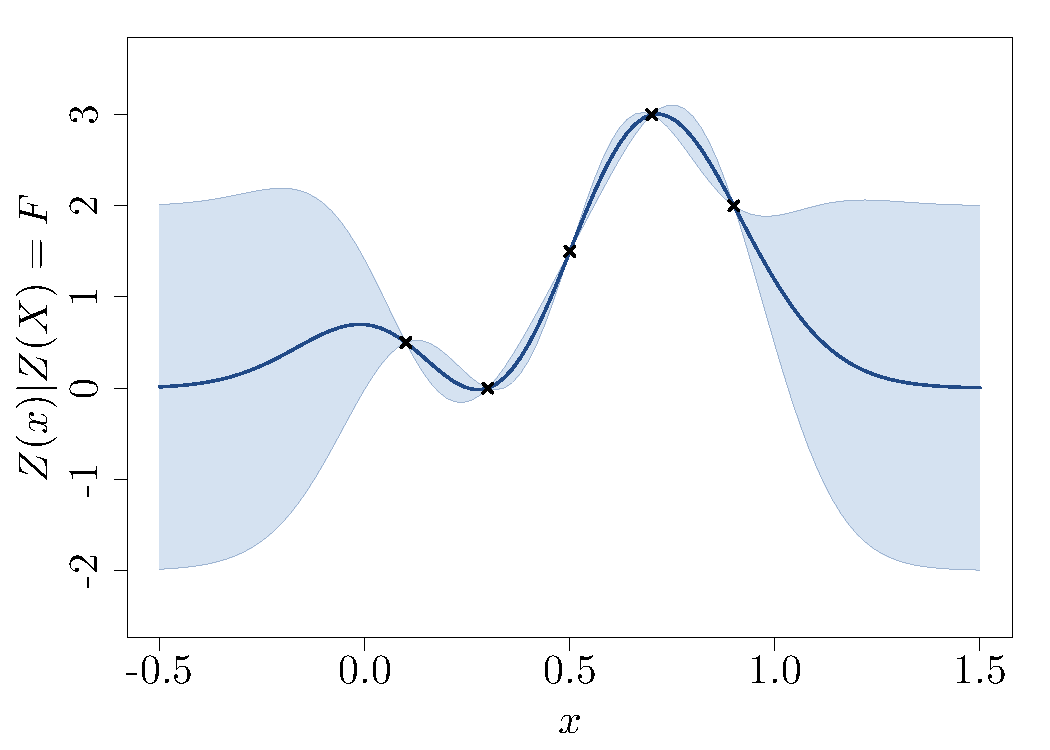
\includegraphics[height=5cm]{figures/python/GPR}
\end{center}
\begin{equation*}
	\begin{split}
		m(x) &= k(x,X)k(X,X)^{-1}F\\
		c(x,y) &= k(x,y) - k(x,X)k(X,X)^{-1}k(X,y)
	\end{split}
\end{equation*}
\\ \ \\
We will discuss these models in more details today.
\end{frame}

%%%%%%%%%%%%%%%%%%%%%%%%%%%%%%%%%%%%%%%%%%%%%%%%%%%%%%
\begin{frame}{}
Outline of todays lecture
\vspace{0.2cm}
\begin{itemize}
	\item Parameters estimation
	\item Model validation
	\item Kernel designs
	\item ``Exotic'' informations
\end{itemize}
\end{frame}

%%%%%%%%%%%%%%%%%%%%%%%%%%%%%%%%%%%%%%%%%%%%%%%%%%%%%%
%%%%%%%%%%%%%%%%%%%%%%%%%%%%%%%%%%%%%%%%%%%%%%%%%%%%%%
\section[Param. estim.]{Parameter estimation}
\subsection{}

%%%%%%%%%%%%%%%%%%%%%%%%%%%%%%%%%%%%%%%%%%%%%%%%%%%%%%
\begin{frame}{}
We have seen previously that the choice of the kernel and its parameters have a great influence on the model. \\ \vspace{5mm}
In order to choose a prior that is suited to the data at hand, we can consider:
\begin{itemize}
	\item minimising the model error
	\item Using maximum likelihood estimation 
\end{itemize}
We will now detail the second one.
\end{frame}

%%%%%%%%%%%%%%%%%%%%%%%%%%%%%%%%%%%%%%%%%%%%%%%%%%%%%%
\begin{frame}{}
\begin{definition}
The \textbf{likelihood} of a distribution with a density $f_X$ given some observations $X_1, \dots,X_p$ is:
\begin{equation*}
 	L = \prod_{i=1}^p f_X(X_i)
\end{equation*} 
\end{definition}
This quantity can be used to measure the adequacy between observations and a distribution.\\ \vspace{3mm}
\end{frame}

%%%%%%%%%%%%%%%%%%%%%%%%%%%%%%%%%%%%%%%%%%%%%%%%%%%%%%
\begin{frame}{}
In the GPR context, we often have only \textbf{one observation} of the vector $F$. The likelihood is then:
\begin{equation*}
 	L = f_{Z(X)}(F) = \frac{1}{\displaystyle (2 \pi)^{n/2} |k(X,X)|^{1/2}} \exp \left(-\frac12 F^t k(X,X)^{-1} F  \right).
\end{equation*} 
It is thus possible to maximise $L$ -- or $\log(L)$ -- with respect to the kernel's parameters in order to find a well suited prior. 
\end{frame}

%%%%%%%%%%%%%%%%%%%%%%%%%%%%%%%%%%%%%%%%%%%%%%%%%%%%%%
\begin{frame}{}
\begin{example}
	We consider 100 sample from a  Matern 5/2 process with parameters $\sigma^2=1$ and $\theta = 0.2$, and $n$ observation points. We then try to recover the kernel parameters using MLE.\\ \vspace{5mm}
	\centering
	\begin{tabular}{|c|cccc|}
		\hline
		$n$ & 5 & 10 & 15 & 20 \\ \hline
		$\sigma^2$ & 1.0 (0.7) & 1.11 (0.71) & 1.03 (0.73) & 0.88 (0.60) \\
		$\theta$ & 0.20 (0.13) & 0.21 (0.07) & 0.20 (0.04) & 0.19 (0.03) \\ \hline
	\end{tabular}
\end{example}
\vspace{5mm}
MLE can be applied regardless to the dimension of the input space.
\end{frame}

%%%%%%%%%%%%%%%%%%%%%%%%%%%%%%%%%%%%%%%%%%%%%%%%%%%%%%
%%%%%%%%%%%%%%%%%%%%%%%%%%%%%%%%%%%%%%%%%%%%%%%%%%%%%%
\section{Model validation}
\subsection{}

%%%%%%%%%%%%%%%%%%%%%%%%%%%%%%%%%%%%%%%%%%%%%%%%%%%%%%
\begin{frame}{}
We have seen that given some observations $F=f(X)$, it is very easy to build lots of models, either by changing the kernel parameters or the kernel itself.\\ \vspace{5mm}
The interesting question now is to know how to get a good model. To do so, we will need to answer the following questions:
\begin{itemize}
	\item What is a good model?
	\item How to measure it?
\end{itemize}
\end{frame}

%%%%%%%%%%%%%%%%%%%%%%%%%%%%%%%%%%%%%%%%%%%%%%%%%%%%%%
\begin{frame}{}
The idea is to introduce new data and to compare the model prediction with reality 
\begin{center}
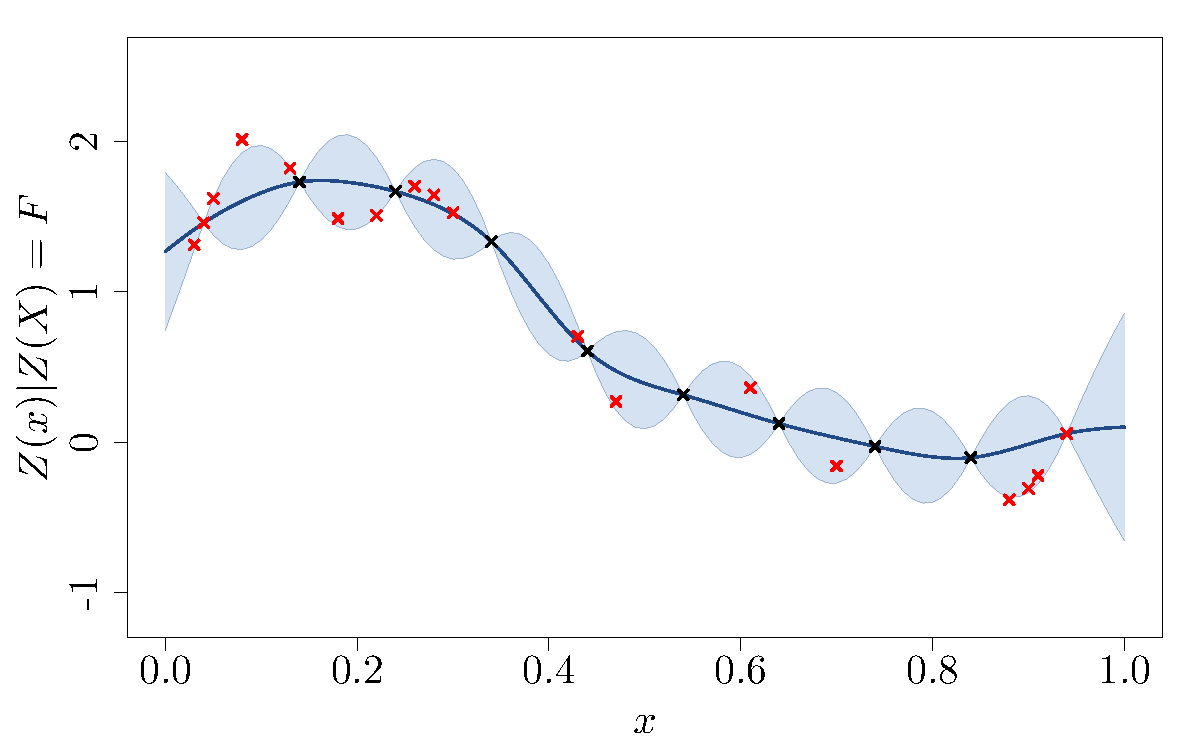
\includegraphics[height=4.5cm]{figures/R/VALID_testset}
\end{center}
\vspace{3mm}
Since GPR models provide a mean and a covariance structure for the error they both have to be assessed.
\end{frame}

%%%%%%%%%%%%%%%%%%%%%%%%%%%%%%%%%%%%%%%%%%%%%%%%%%%%%%
\begin{frame}{}
Let $X_t$ be the test set and $F_t=f(X_t)$ be the associated observations.\\ \vspace{5mm}
The accuracy of the mean can be measured by computing: 
\begin{equation*}
	\begin{split}
		\text{Mean Square Error\qquad}& MSE = \mathrm{mean} ((F_t - m(X_t))^2) \\
		\text{A ``normalised'' criterion\qquad}& Q_2 = 1 - \frac{\sum (F_t - m(X_t))^2}{\sum (F_t - \mathrm{mean}(F_t))^2} 
	\end{split}
\end{equation*}
\\ \ \\
On the above example we get $MSE = 0.038$ and $Q_2 = 0.95$.
\end{frame}

%%%%%%%%%%%%%%%%%%%%%%%%%%%%%%%%%%%%%%%%%%%%%%%%%%%%%%
\begin{frame}{}
The predicted distribution can be tested by normalising the residuals. \\ \vspace{3mm}
According to the model, $F_t \sim \mathcal{N}(m(X_t),c(X_t,X_t))$.\\ \vspace{3mm}
$c(X_t,X_t)^{-1/2}(F_t-m(X_t)) $ should thus be independents $\mathcal{N}(0,1)$:
\begin{center}
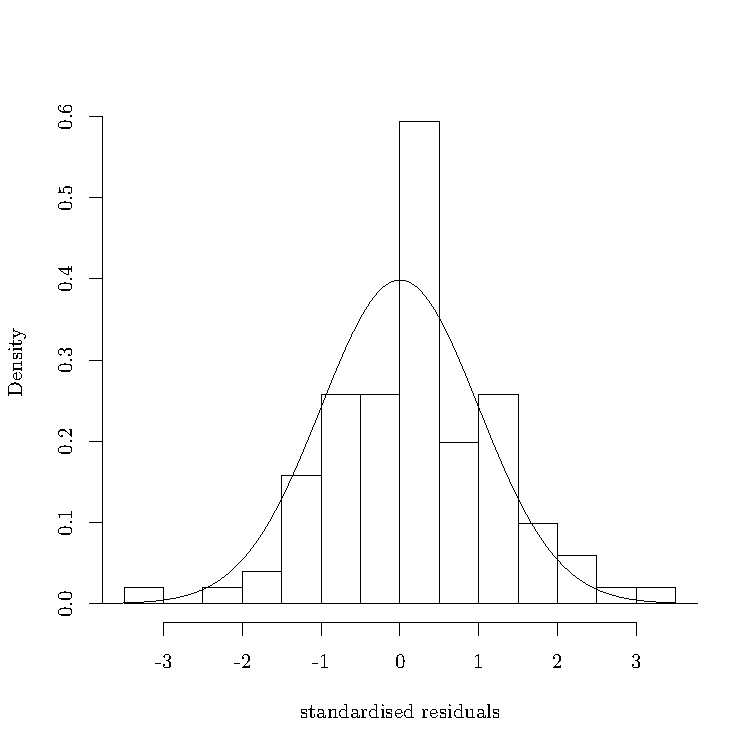
\includegraphics[height=5cm]{figures/R/VALID_hist} \qquad
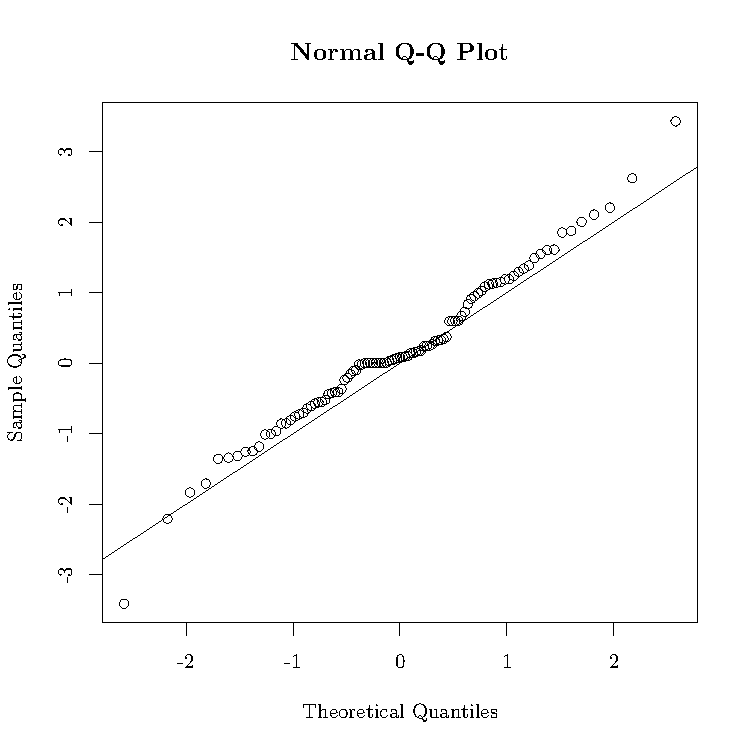
\includegraphics[height=5cm]{figures/R/VALID_qqplot}
\end{center}
\end{frame}

%%%%%%%%%%%%%%%%%%%%%%%%%%%%%%%%%%%%%%%%%%%%%%%%%%%%%%
\begin{frame}{}
When no test set is available, another option is to consider cross validation methods such as leave-one-out. \\ \vspace{5mm}
The steps are:
\begin{enumerate}
	\item[1.] build a model based on all observations except one
	\item[2.] compute the model error at this point
\end{enumerate}
This procedure can be repeated for all the design points in order to get a vector of error.\\ \vspace{3mm}
\end{frame}

%%%%%%%%%%%%%%%%%%%%%%%%%%%%%%%%%%%%%%%%%%%%%%%%%%%%%%
\begin{frame}{}
Model to be tested:\\ \vspace{3mm}
\begin{center}
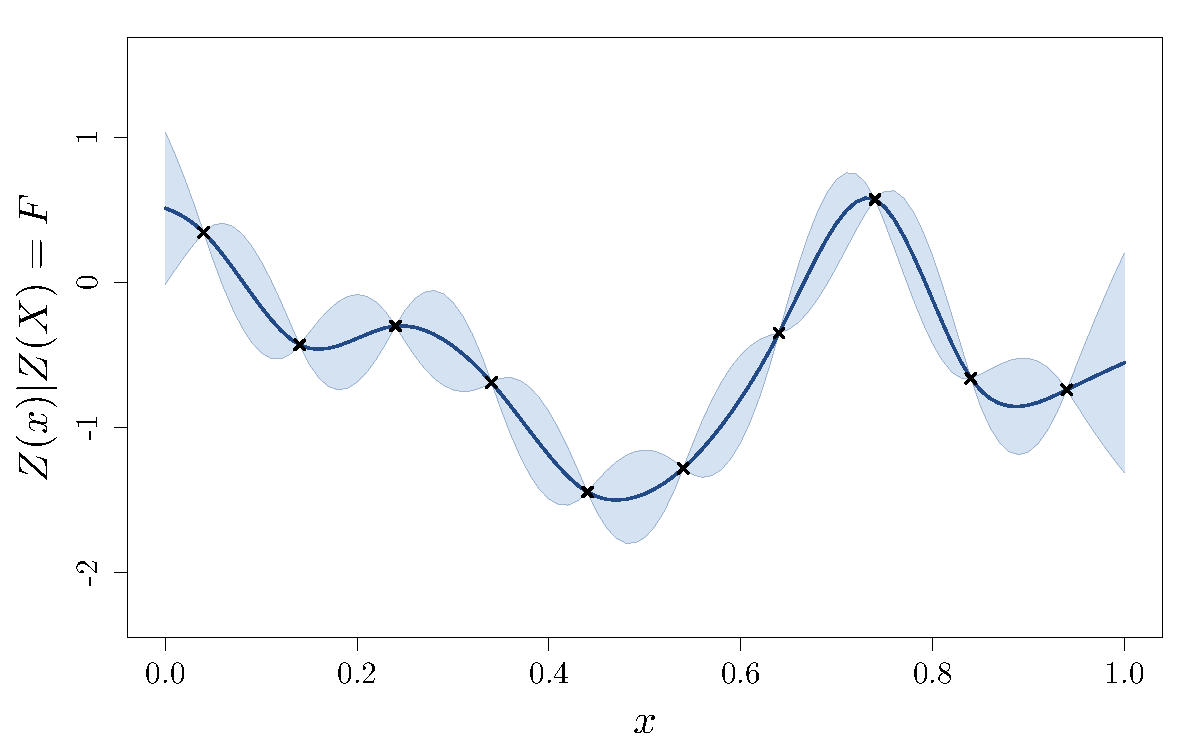
\includegraphics[height=6cm]{figures/R/VALID_crossval0}
\end{center}
\end{frame}

%%%%%%%%%%%%%%%%%%%%%%%%%%%%%%%%%%%%%%%%%%%%%%%%%%%%%%
\begin{frame}{}
Step 1:\\ \vspace{3mm}
\begin{center}
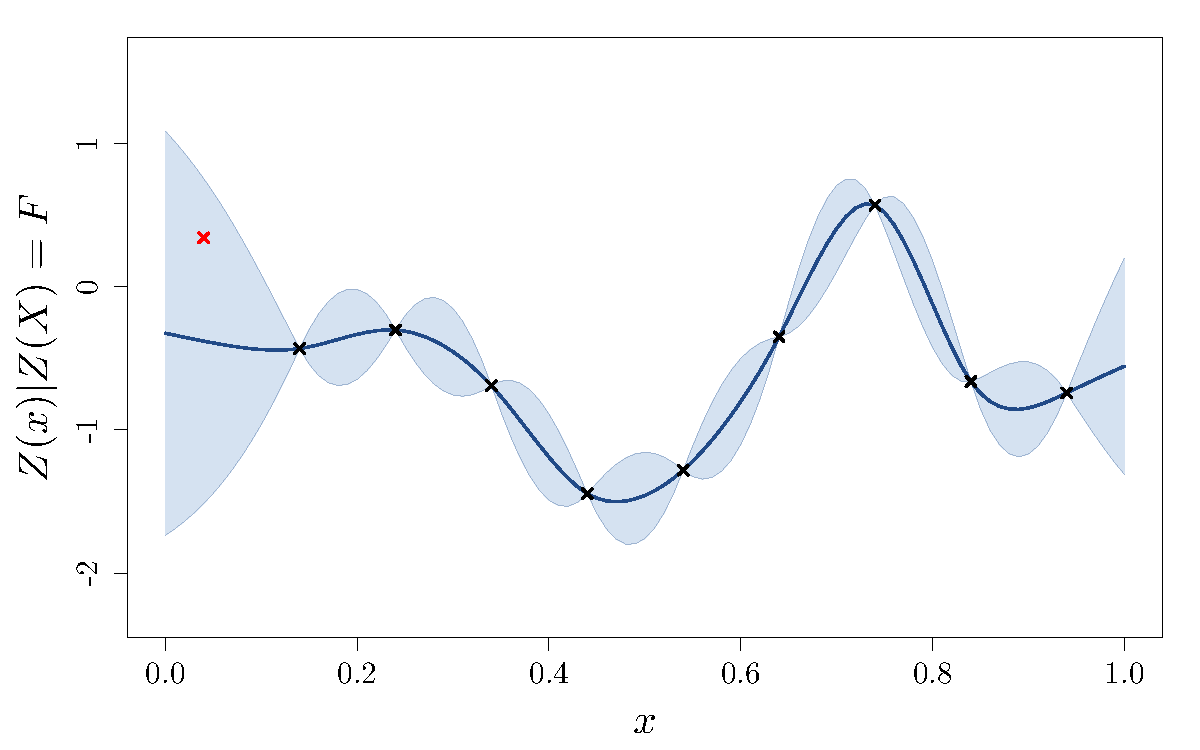
\includegraphics[height=6cm]{figures/R/VALID_crossval1}
\end{center}
\end{frame}

%%%%%%%%%%%%%%%%%%%%%%%%%%%%%%%%%%%%%%%%%%%%%%%%%%%%%%
\begin{frame}{}
Step 2:\\ \vspace{3mm}
\begin{center}
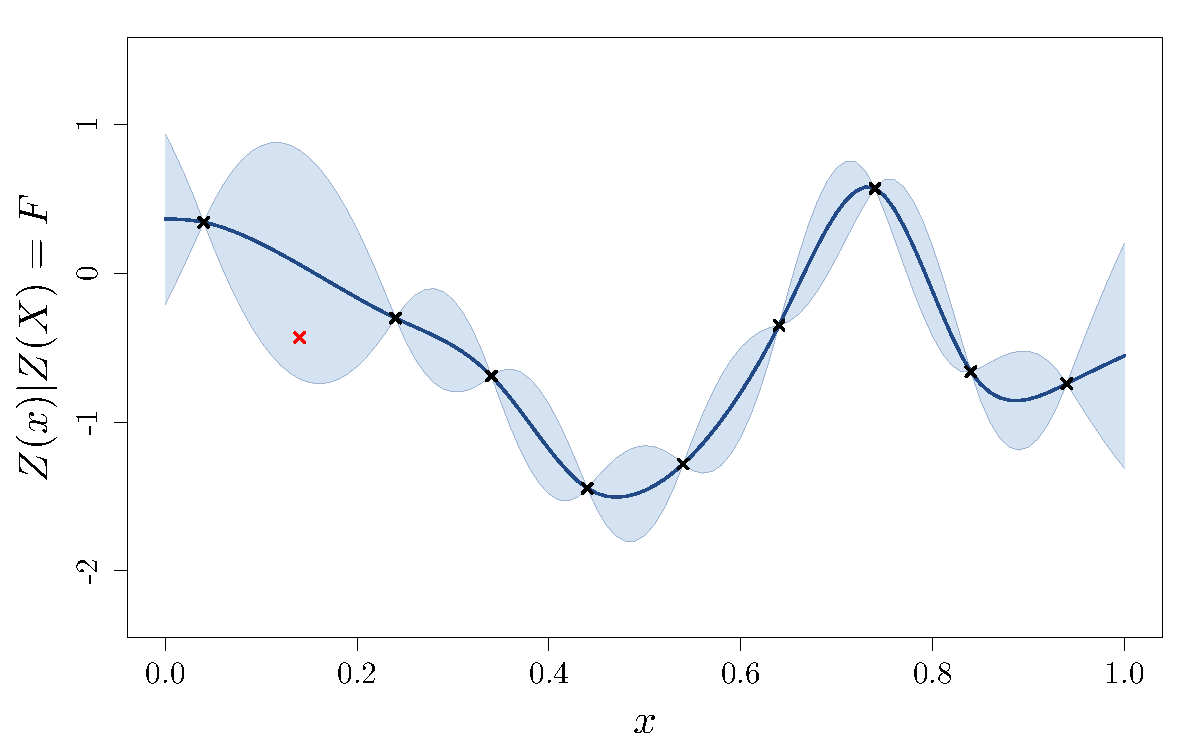
\includegraphics[height=6cm]{figures/R/VALID_crossval2}
\end{center}
\end{frame}

%%%%%%%%%%%%%%%%%%%%%%%%%%%%%%%%%%%%%%%%%%%%%%%%%%%%%%
\begin{frame}{}
Step 3:\\ \vspace{3mm}
\begin{center}
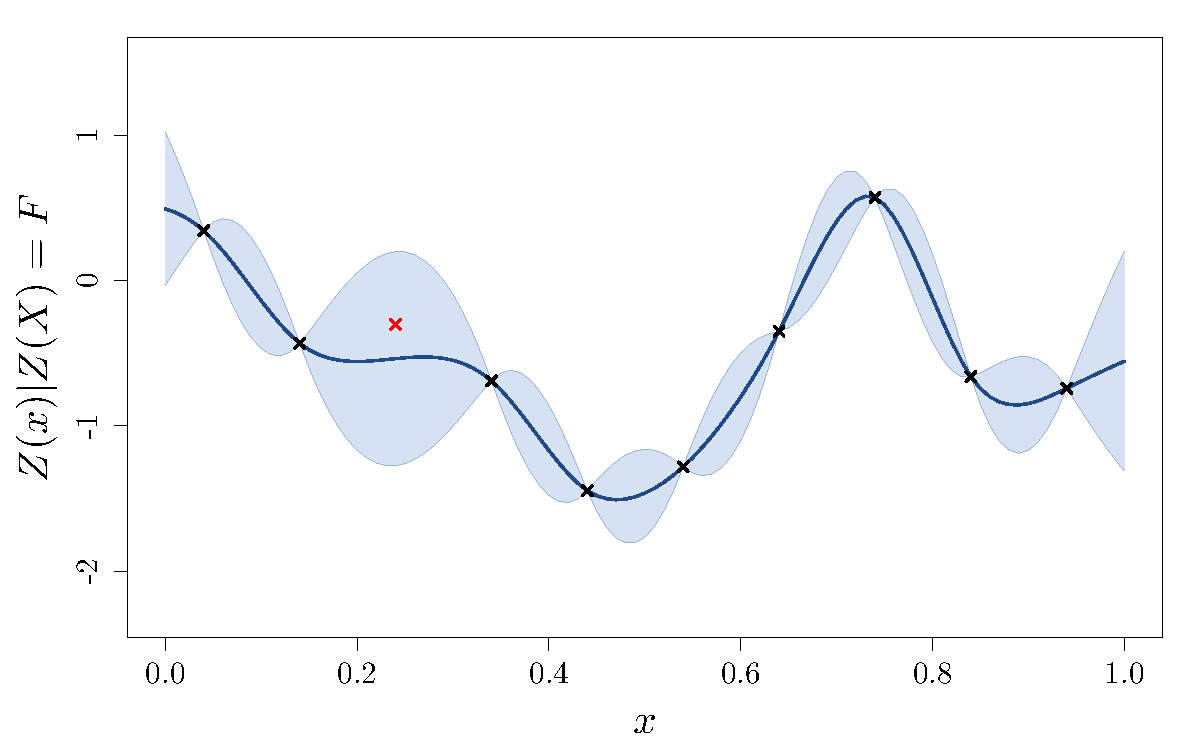
\includegraphics[height=6cm]{figures/R/VALID_crossval3}
\end{center}
\end{frame}

%%%%%%%%%%%%%%%%%%%%%%%%%%%%%%%%%%%%%%%%%%%%%%%%%%%%%%
\begin{frame}{}
If we apply LOO to previous example we obtain:
 $$MSE = 0.24 \text{ and } Q_2 = 0.34.$$
Why doesn't the model perform as good as previously?\\
\vspace{5mm}
\pause
It turns out that errors are always computed at the `worst' location!
\begin{center}
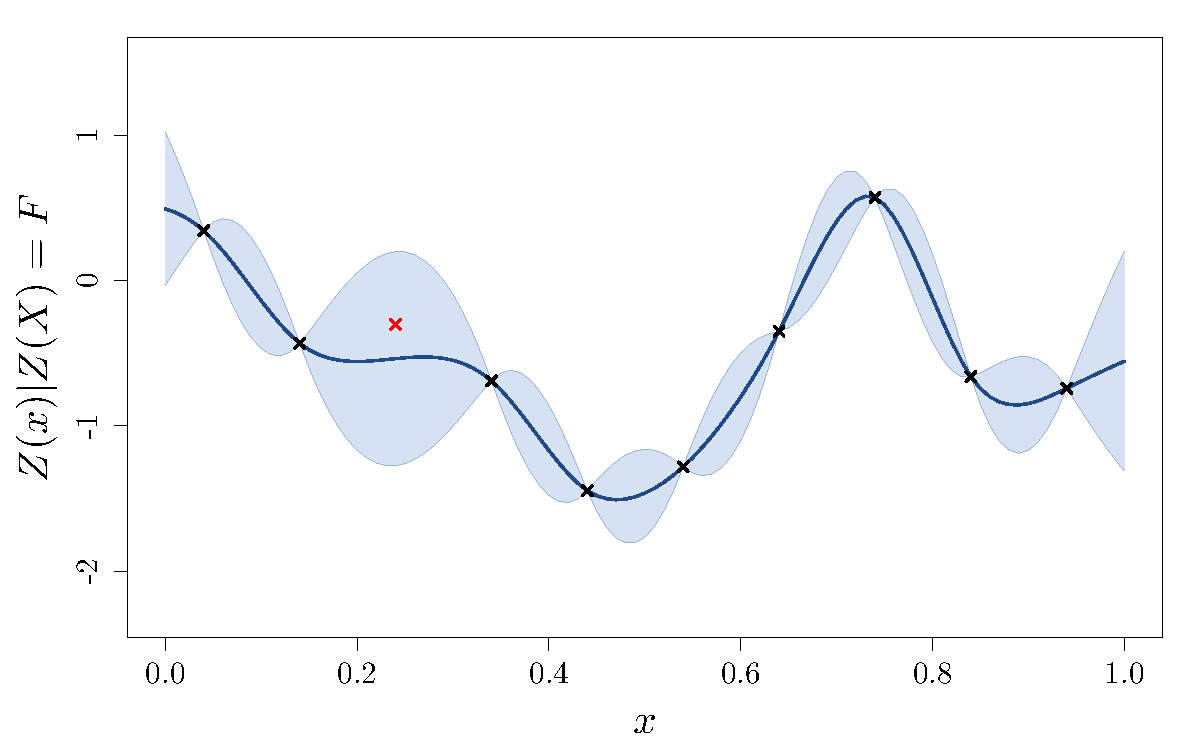
\includegraphics[height=5cm]{figures/R/VALID_crossval3}
\end{center}
\end{frame}

%%%%%%%%%%%%%%%%%%%%%%%%%%%%%%%%%%%%%%%%%%%%%%%%%%%%%%
\begin{frame}{}
We can also look at the residual distribution. For leave-one-out, there is no joint distribution for the residuals so they have to be standardised independently. We obtain: 
\begin{center}
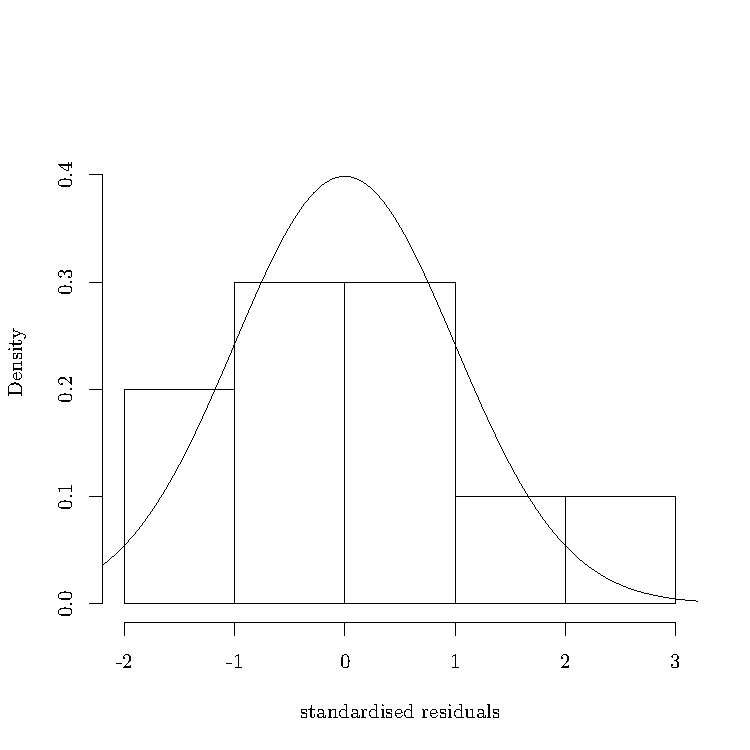
\includegraphics[height=5cm]{figures/R/VALID_crossvalhist} \qquad
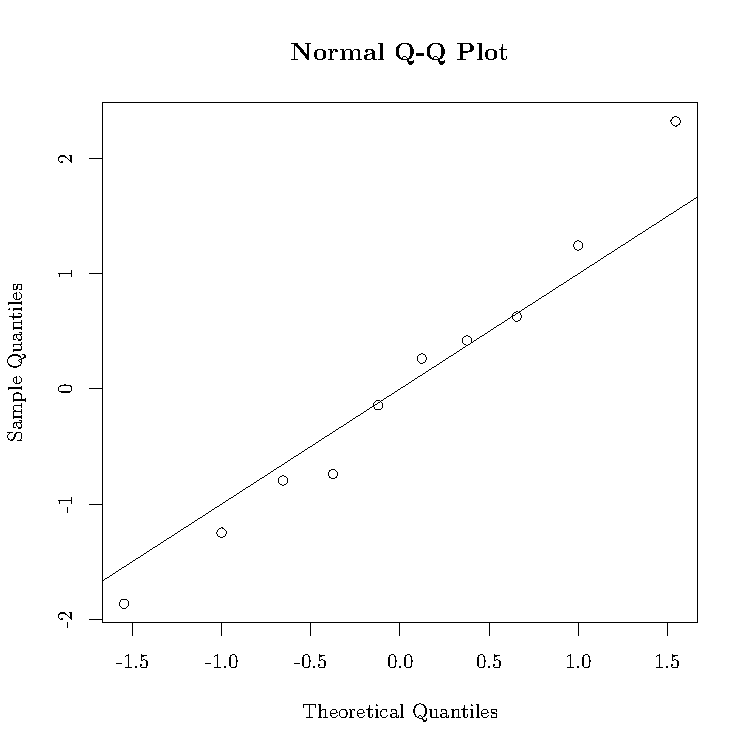
\includegraphics[height=5cm]{figures/R/VALID_crossvalqqplot}
\end{center}
\end{frame}


%%%%%%%%%%%%%%%%%%%%%%%%%%%%%%%%%%%%%%%%%%%%%%%%%%%%%%%%%%%%%%%%%%%%%%%%%%%%%%%%%%%%
%%%%%%%%%%%%%%%%%%%%%%%%%%%%%%%%%%%%%%%%%%%%%%%%%%%%%%%%%%%%%%%%%%%%%%%%%%%%%%%%%%%%
\section{Making new from old}
\subsection{}

%%%%%%%%%%%%%%%%%%%%%%%%%%%%%%%%%%%%%%%%%%%%%%%%%%%%%%
\begin{frame}{}
\structure{Making new from old:}
Many operations can be applied to psd functions while retaining this property
\begin{block}{}
Kernels can be:
\begin{itemize}
  \item Summed together
  \begin{itemize}
    \item On the same space $k(x,y) = k_1(x,y) + k_2(x,y)$
    \item On the tensor space $k(x,y) = k_1(x_1,y_1) + k_2(x_2,y_2)$
  \end{itemize} 
  \item Multiplied together
  \begin{itemize}
    \item On the same space $k(x,y) = k_1(x,y) \times k_2(x,y)$
    \item On the tensor space $k(x,y) = k_1(x_1,y_1) \times k_2(x_2,y_2)$
  \end{itemize} 
  \item Composed with a function
  \begin{itemize}
    \item $k(x,y) = k_1(f(x),f(y))$
  \end{itemize} 
\end{itemize} 
\end{block}
\begin{center}
\alert{How can this be useful?}
\end{center}
\end{frame}

% \subsection{Sum of kernels}

%%%%%%%%%%%%%%%%%%%%%%%%%%%%%%%%%%%%%%%%%%%%%%%%%%%%%%
\begin{frame}{Sum of kernels over the same space }
\begin{example}[The Mauna Loa observatory dataset]
This famous dataset compiles the monthly $CO_2$ concentration in Hawaii since 1958.
\begin{center}
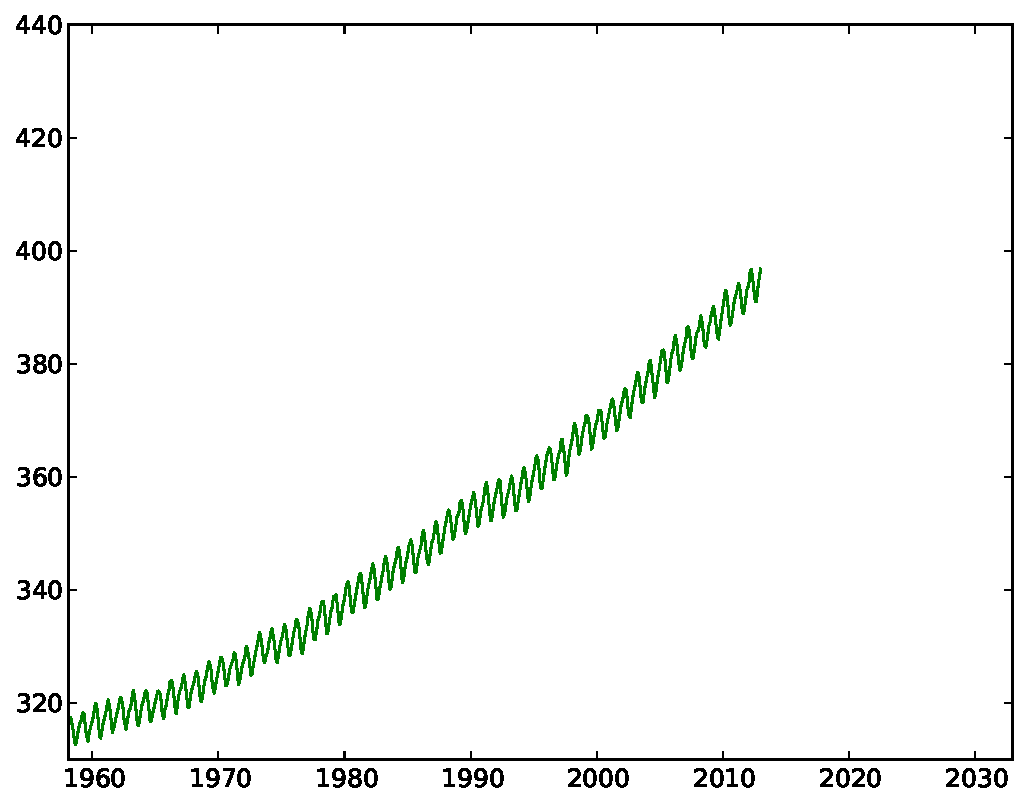
\includegraphics[height=4.5cm]{figures/python/CO2-data}
\end{center}
Let's try to predict the concentration for the next 20 years.
\end{example}
\end{frame}

%%%%%%%%%%%%%%%%%%%%%%%%%%%%%%%%%%%%%%%%%%%%%%%%%%%%%%
\begin{frame}{Sum of kernels over the same space }
We first consider a squared-exponential kernel: 
$$ \displaystyle k(x,y) = \sigma^2\exp \left(-\frac{(x-y)^2}{\theta^2} \right)$$
\begin{center}
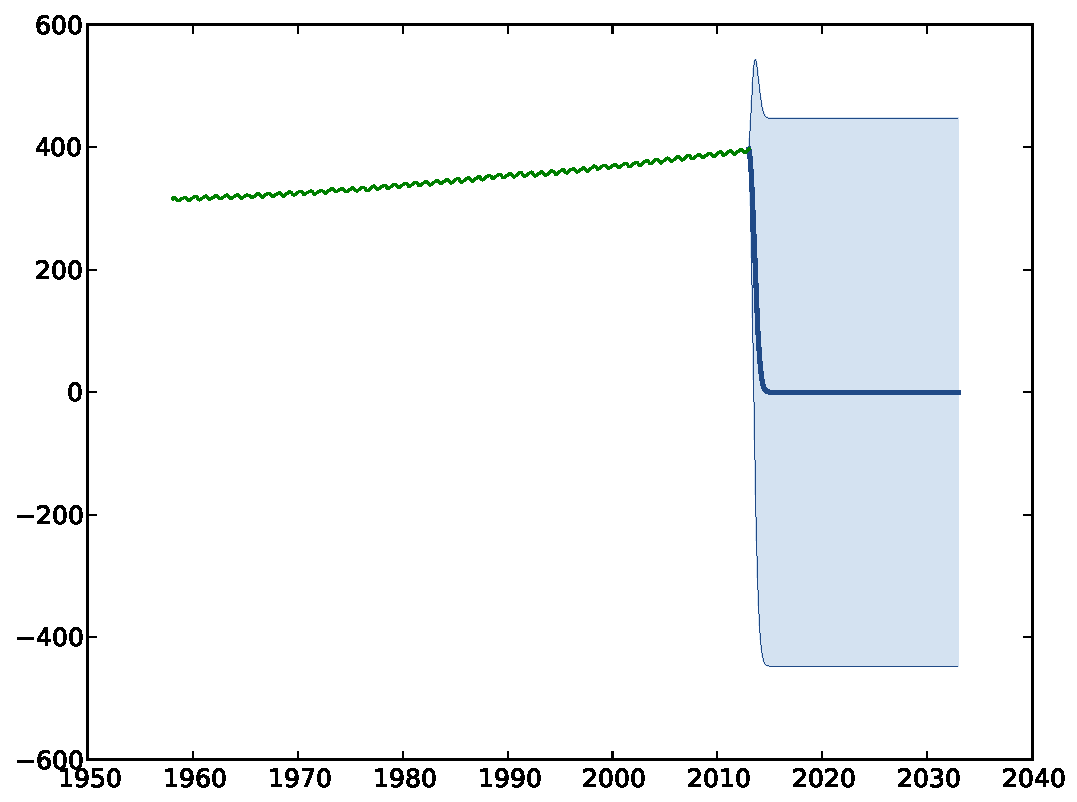
\includegraphics[height=3.7cm]{figures/python/CO2-rbfa} \quad 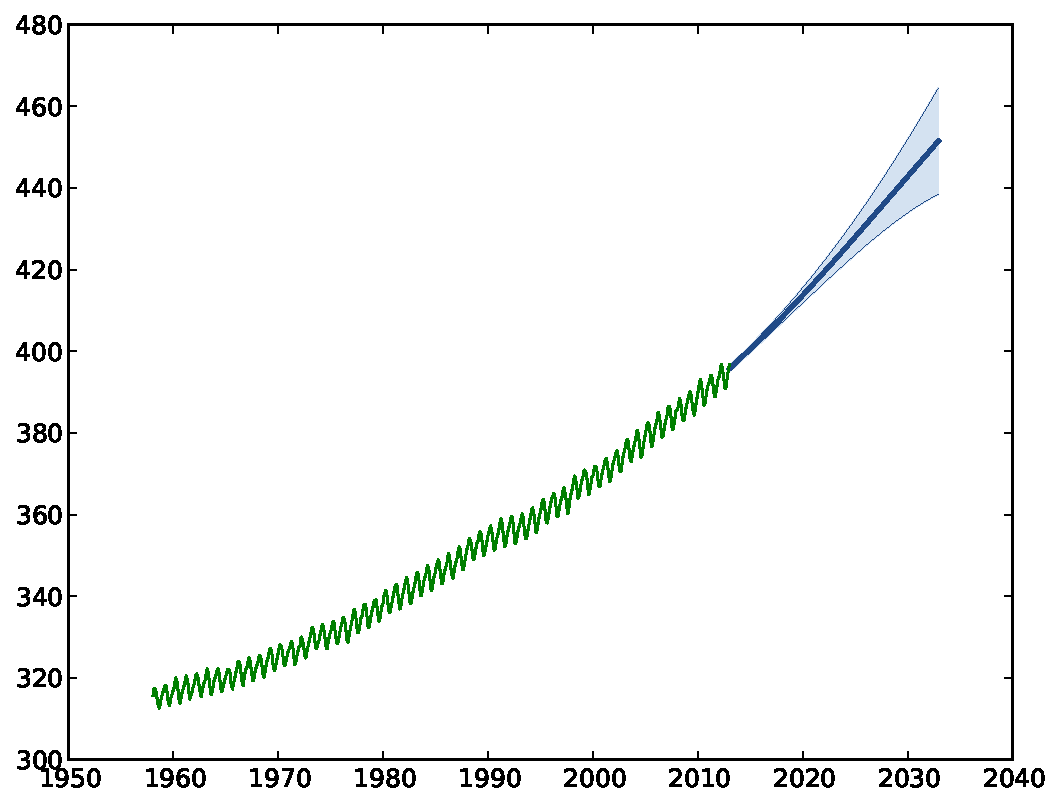
\includegraphics[height=3.7cm]{figures/python/CO2-rbfb}
\end{center}
\begin{block}{}
\centering
\alert{The results are terrible!}
\end{block}
\end{frame}

%%%%%%%%%%%%%%%%%%%%%%%%%%%%%%%%%%%%%%%%%%%%%%%%%%%%%%
\begin{frame}{Sum of kernels over the same space }
What happen if we sum both kernels?
\begin{equation*}
k(x,y) = k_{rbf1}(x,y) + k_{rbf2}(x,y)
\end{equation*} 
\pause
\begin{center}
\vspace{-8mm} 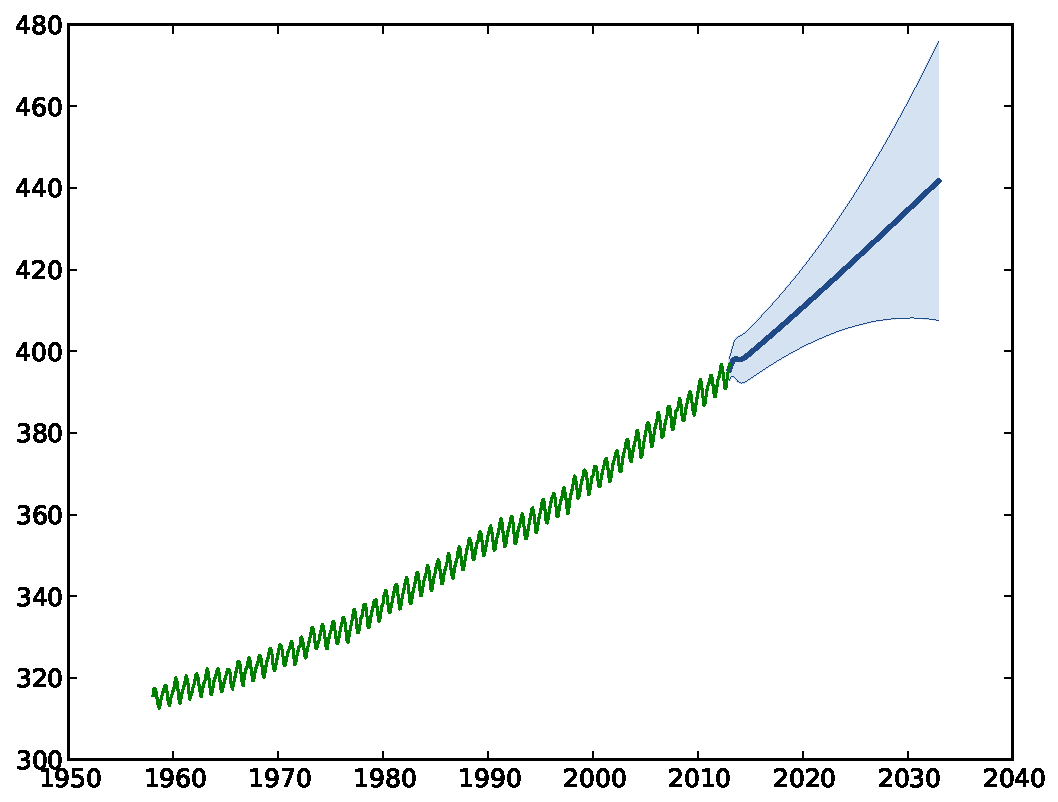
\includegraphics[height=4.5cm]{figures/python/CO2-rbfab}
\end{center}
%\vspace{1mm}
\begin{block}{}
\centering
\alert{The model is drastically improved!}
\end{block}
\end{frame}

%%%%%%%%%%%%%%%%%%%%%%%%%%%%%%%%%%%%%%%%%%%%%%%%%%%%%%
\begin{frame}{Sum of kernels over the same space }
We can try the following kernel:
\begin{equation*}
k(x,y) = \sigma_0^2  x^2 y^2 + k_{rbf1}(x,y) + k_{rbf2}(x,y) + k_{per}(x,y)
\end{equation*}
\pause
\begin{center}
\vspace{-8mm}  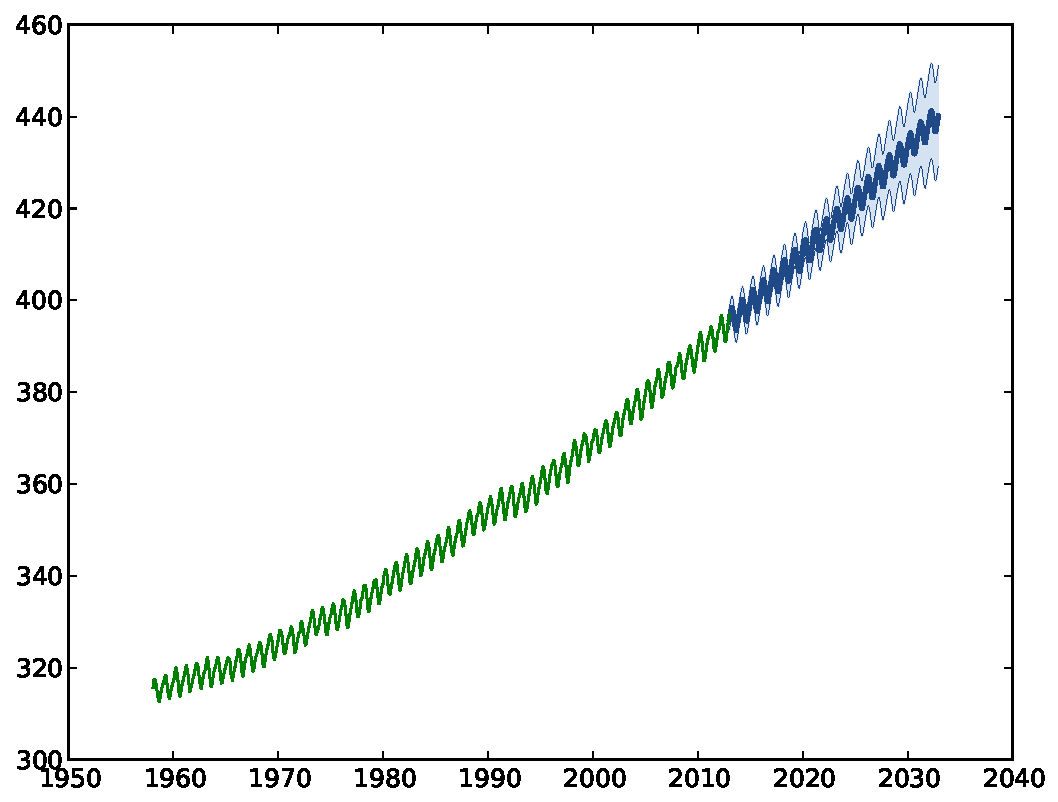
\includegraphics[height=4.5cm]{figures/python/CO2-rbfabpq}
\end{center}
\begin{block}{}
\centering
\alert{Once again, the model is significantly improved.}
\end{block}
\end{frame}


%%%%%%%%%%%%%%%%%%%%%%%%%%%%%%%%%%%%%%%%%%%%%%%%%%%%%%
\begin{frame}{Sum of kernels over tensor space}
\begin{block}{Property}
\begin{equation*}
k(x,y) = k_1(x_1,y_1) +  k_2(x_2,y_2)
\end{equation*}
is valid covariance structure.\\
\begin{columns}[c]
\begin{column}{3cm}
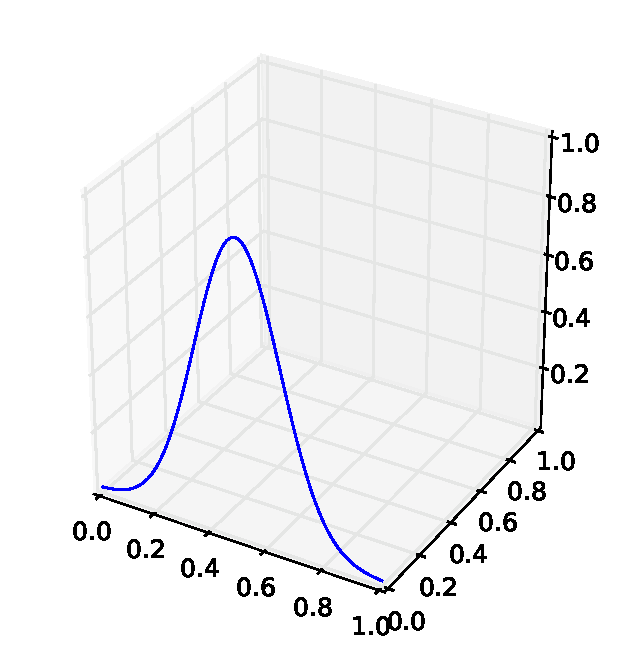
\includegraphics[width=3cm]{figures/python/newfromold-sum2-k1}
\end{column}
\begin{column}{2mm}
$+$
\end{column}
\begin{column}{3cm}
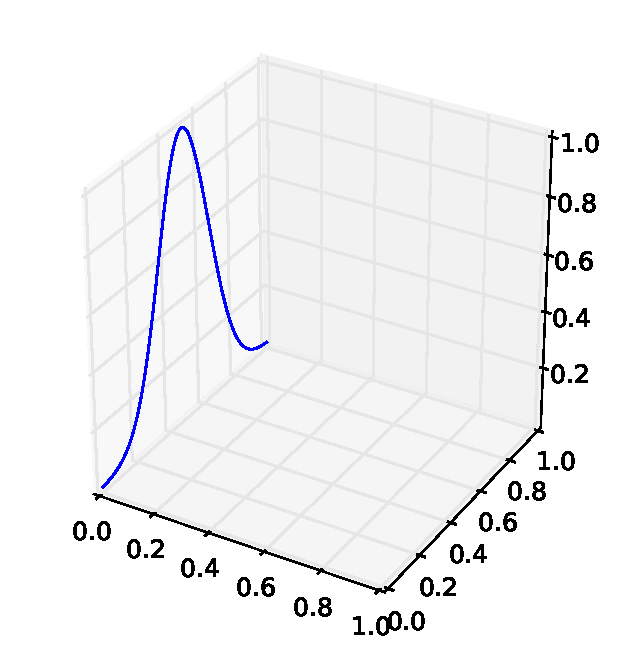
\includegraphics[width=3cm]{figures/python/newfromold-sum2-k2}
\end{column}
\begin{column}{2mm}
$=$
\end{column}
\begin{column}{3cm}
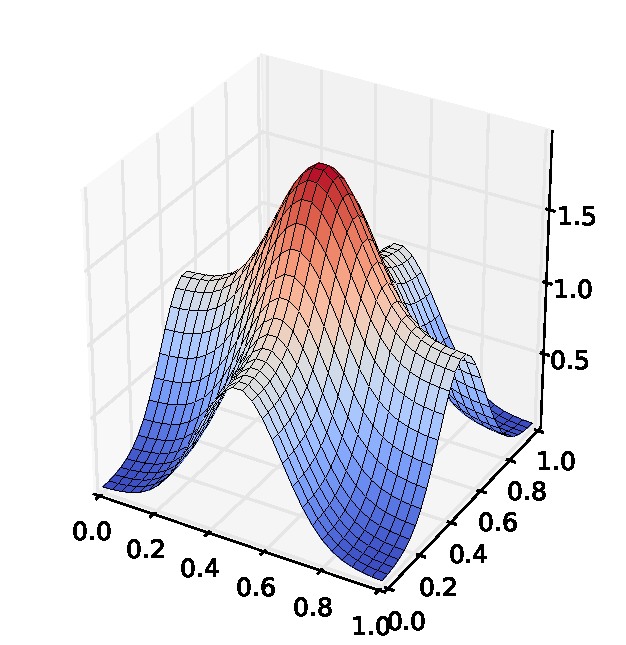
\includegraphics[width=3cm]{figures/python/newfromold-sum2-k12}
\end{column}
\end{columns}
\vspace{4mm}
\end{block}
\structure{Remark:}
From a GP point of view, $k$ is the kernel of 
$$Z(x) = Z_1(x_1) + Z_2(x_2)$$
\end{frame}

%%%%%%%%%%%%%%%%%%%%%%%%%%%%%%%%%%%%%%%%%%%%%%%%%%%%%%
\begin{frame}{Sum of kernels over tensor space}
We can have a look at a few sample paths from $Z$:
\begin{center}
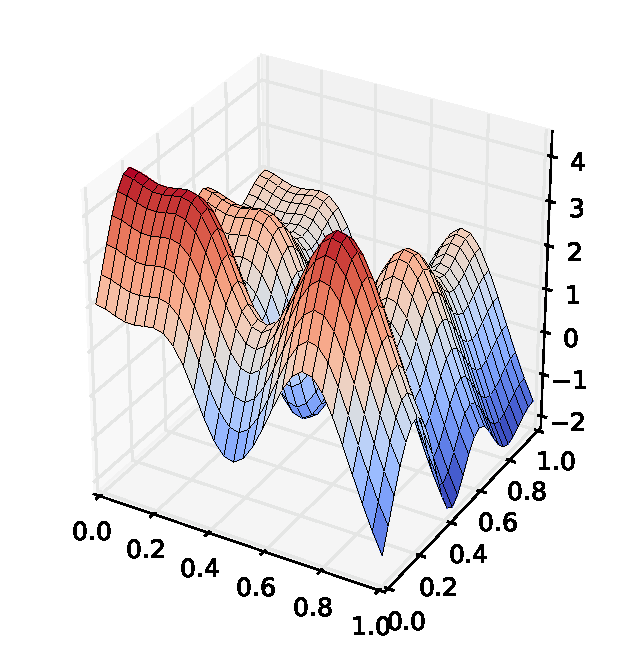
\includegraphics[width=3.5cm]{figures/python/newfromold-sum2-traj124} 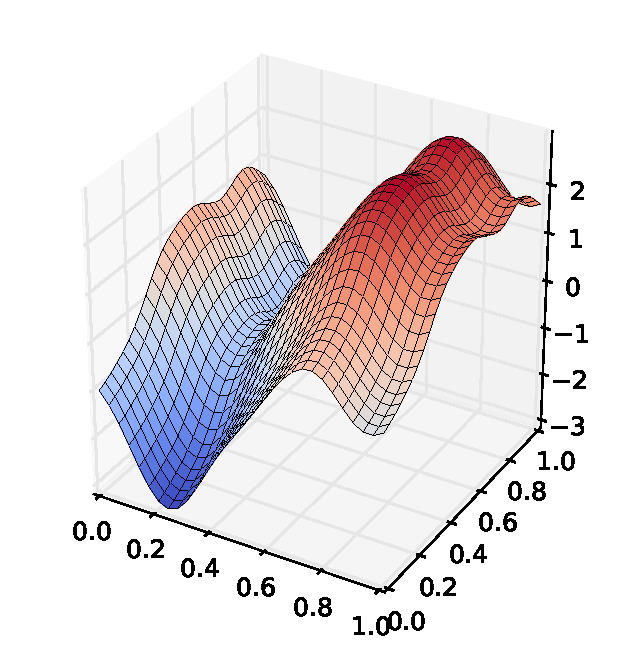
\includegraphics[width=3.5cm]{figures/python/newfromold-sum2-traj121} 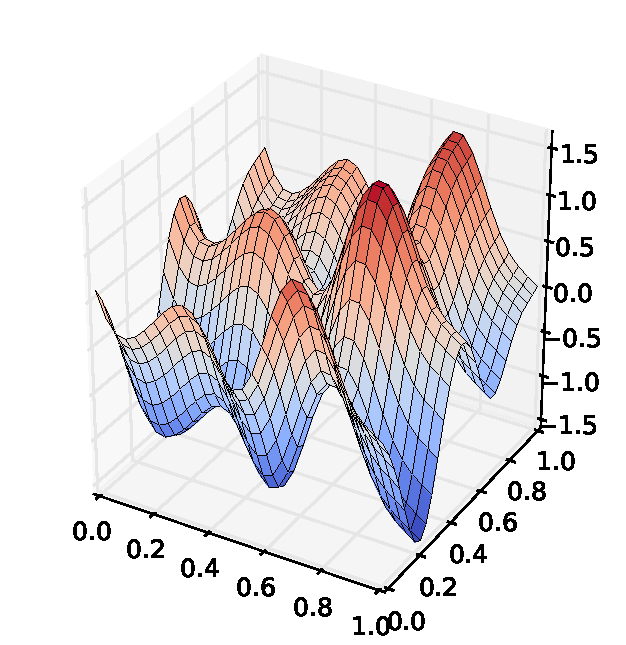
\includegraphics[width=3.5cm]{figures/python/newfromold-sum2-traj123} % 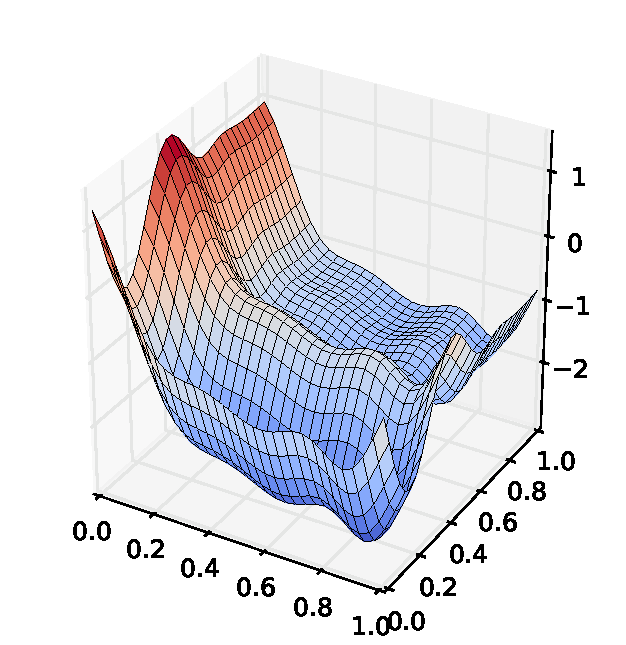
\includegraphics[width=3.5cm]{Figures/newfromold-sum2-traj122} 
\end{center}
\qquad \alert{$\Rightarrow$ They are additive (up to a modification)}\\ \ \\
Tensor Additive kernels are very useful for
\begin{itemize}
  \item Approximating additive functions
  \item Building models over high dimensional inputs spaces
\end{itemize}
\end{frame}

%%%%%%%%%%%%%%%%%%%%%%%%%%%%%%%%%%%%%%%%%%%%%%%%%%%%%%
\begin{frame}{Sum of kernels over tensor space}
We consider the test function $f(x) = \sin( 4 \pi x_1) + \cos( 4 \pi x_2) + 2 x_2$ and a set of 20 observation in $[0,1]^2$. \\ \vspace{5mm}
\begin{columns}[c]
\begin{column}{5cm}
\textbf{Test function}
\begin{center}
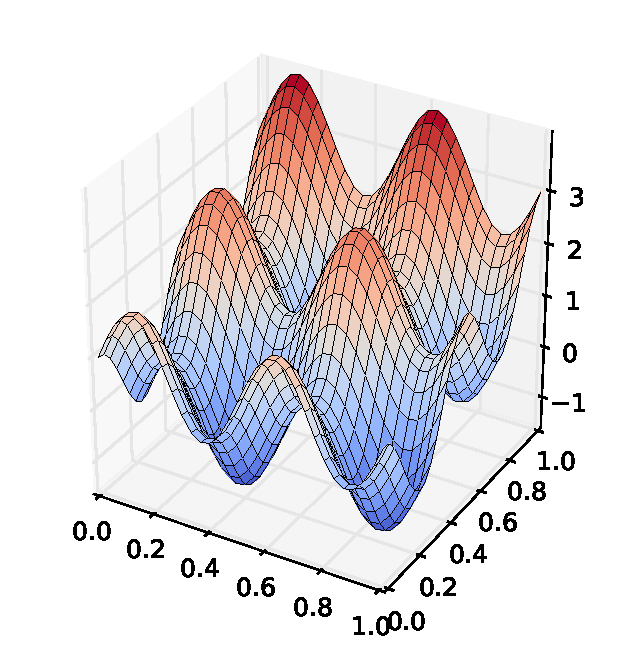
\includegraphics[height=4cm]{figures/python/newfromold-productvssum2-predt}
\end{center}
\end{column}
\begin{column}{5cm}
\textbf{Observations}
\begin{center}
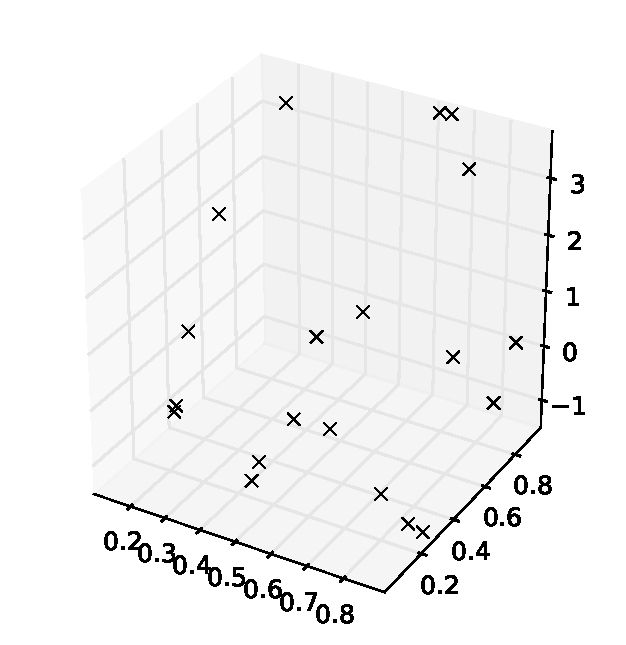
\includegraphics[height=4cm]{figures/python/newfromold-productvssum2-preddoe}
\end{center}
\end{column}
\end{columns} 
\vspace{5mm}
\
\end{frame}

%%%%%%%%%%%%%%%%%%%%%%%%%%%%%%%%%%%%%%%%%%%%%%%%%%%%%%
\begin{frame}{Sum of kernels over tensor space}
We obtain the following models:\\ \vspace{5mm}
\begin{columns}[c]
\begin{column}{5cm}
\textbf{Gaussian kernel}
\begin{center}
Mean predictor
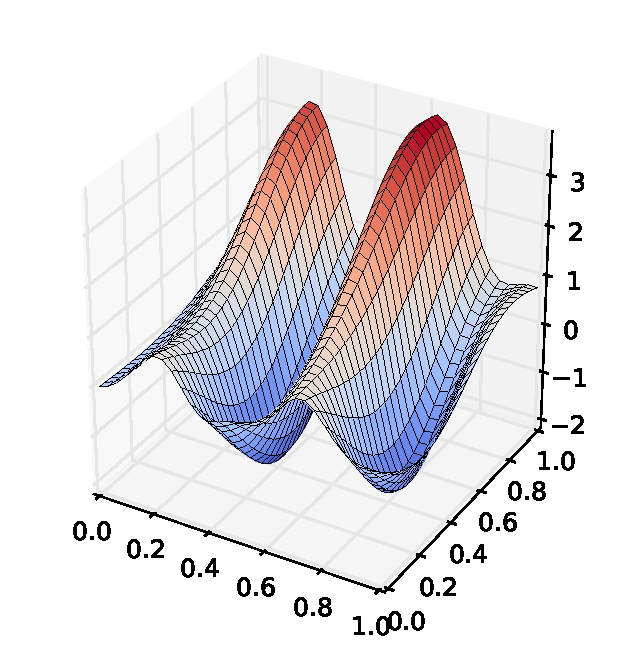
\includegraphics[height=4cm]{figures/python/newfromold-productvssum2-predp}\\
RMSE is 1.06
\end{center}
\end{column}
\begin{column}{5cm}
\textbf{Additive Gaussian kernel}
\begin{center}
Mean predictor
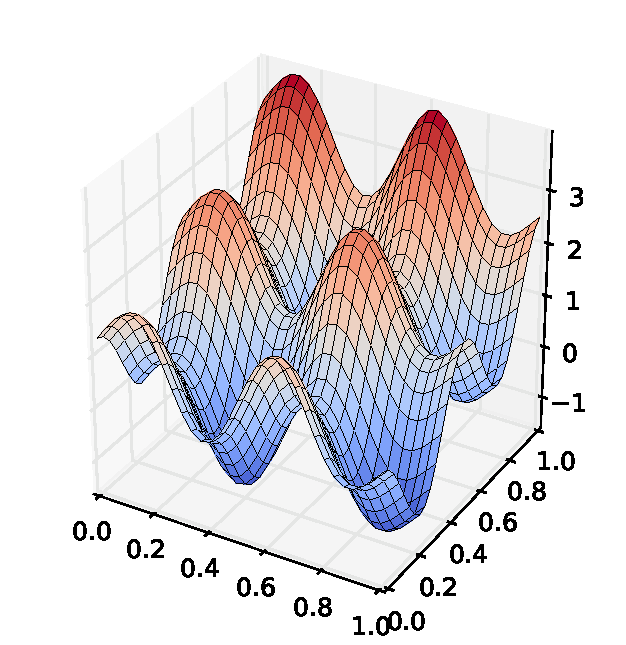
\includegraphics[height=4cm]{figures/python/newfromold-productvssum2-preda}\\
RMSE is 0.12
\end{center}
\end{column}
\end{columns} 
\end{frame}

%%%%%%%%%%%%%%%%%%%%%%%%%%%%%%%%%%%%%%%%%%%%%%%%%%%%%%
\begin{frame}{Sum of kernels over tensor space}
\begin{block}{Remark}%[(continuation)]
\begin{itemize}
\item It is straightforward to show that the mean predictor is additive
\begin{equation*}
\begin{split}
m(x) & = (k_1(x_1,X_1)+k_2(x_2,X_2)) k(X,X)^{-1} F \\
& = \underbrace{k_1(x_1,X_1) k(X,X)^{-1} F}_{m_1(x_1)} + \underbrace{k_2(x_2,X_2) k(X,X)^{-1} F}_{m_2(x_2)}
\end{split}
\end{equation*}
\end{itemize}
\end{block}
\vspace{5mm}
\begin{block}{}
\alert{ $\Rightarrow$ The mean predictor shares the prior behaviour.}
\end{block}
\vfill \
\vspace{2cm} \
\end{frame}

%%%%%%%%%%%%%%%%%%%%%%%%%%%%%%%%%%%%%%%%%%%%%%%%%%%%%%
\begin{frame}{Sum of kernels over tensor space}
\begin{block}{Remark}%[(continuation)]
\begin{itemize}
\item The prediction variance has interesting features
\begin{columns}[c]
\begin{column}{5cm}
\begin{center}
pred. var. with kernel product
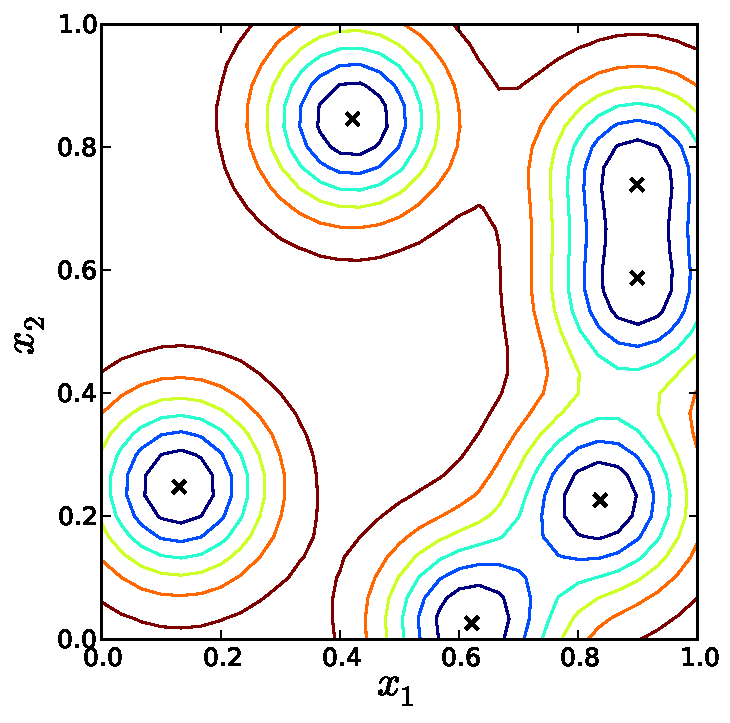
\includegraphics[height=4cm]{figures/python/kernelmodels-predvarprod}
\end{center}
\end{column}
\begin{column}{5cm}
\begin{center}
pred. var. with kernel sum
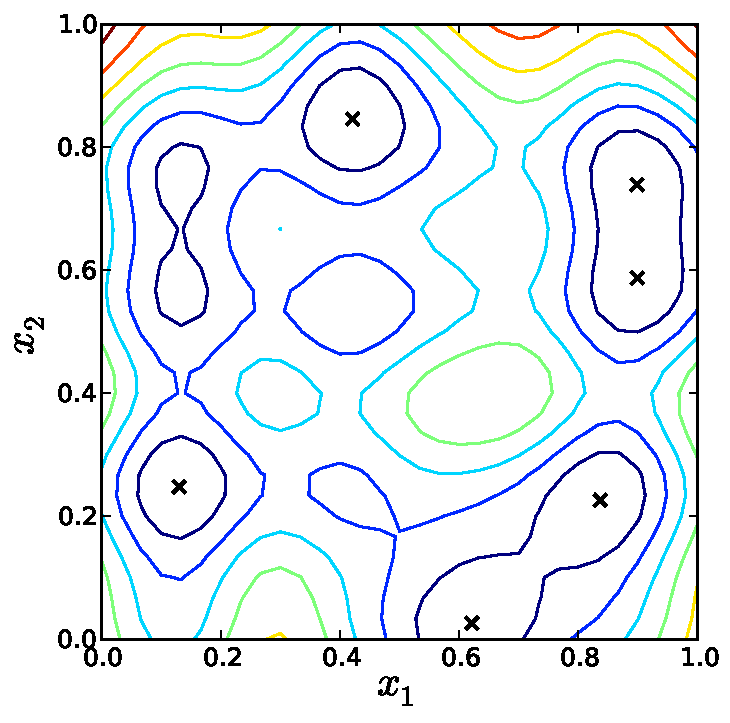
\includegraphics[height=4cm]{figures/python/kernelmodels-predvar}
\end{center}
\end{column}
\end{columns}
\end{itemize} 
\end{block}
\end{frame}

%%%%%%%%%%%%%%%%%%%%%%%%%%%%%%%%%%%%%%%%%%%%%%%%%%%%%%
\begin{frame}{Sum of kernels over tensor space}
This property can be used to construct a design of experiment that covers the space with only $cst \times d$ points.
\begin{center}
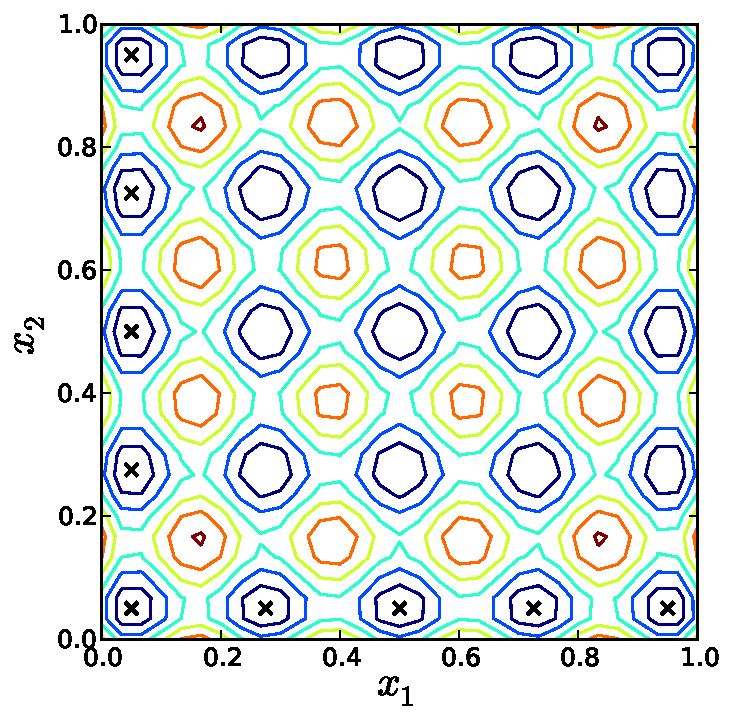
\includegraphics[height=5cm]{figures/python/kernelmodels-predaxe}\\
Prediction variance
\end{center}
\vfill
\end{frame}

% \subsection{Product of kernels}

%%%%%%%%%%%%%%%%%%%%%%%%%%%%%%%%%%%%%%%%%%%%%%%%%%%%%%
\begin{frame}{Product over the same space}
\begin{block}{Property}
\begin{equation*}
k(x,y) = k_1(x,y) \times  k_2(x,y)
\end{equation*}
is valid covariance structure.
\end{block}
%\vspace{10mm}
\begin{example}
We consider the product of a squared exponential with a cosine:
\begin{columns}[c]
\begin{column}{3cm}
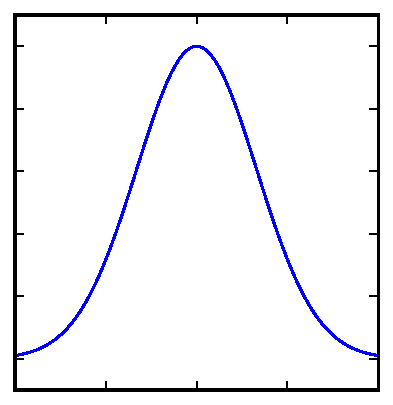
\includegraphics[width=3cm]{figures/python/newfromold-pa.pdf}
\end{column}
\begin{column}{2mm}
$\times$
\end{column}
\begin{column}{3cm}
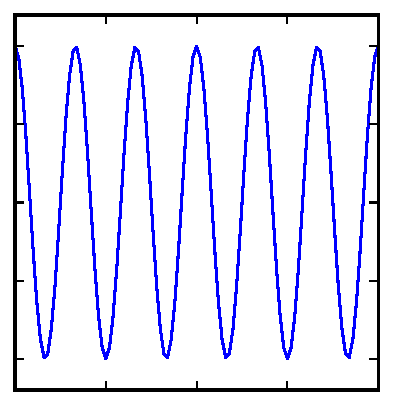
\includegraphics[width=3cm]{figures/python/newfromold-pb.pdf}
\end{column}
\begin{column}{2mm}
$=$
\end{column}
\begin{column}{3cm}
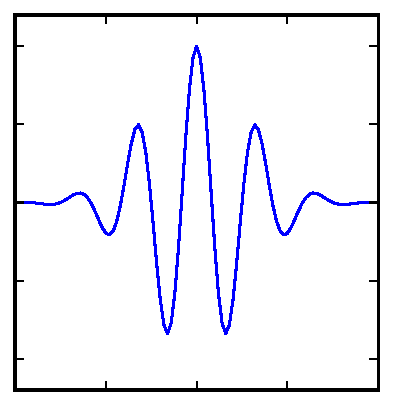
\includegraphics[width=3cm]{figures/python/newfromold-pab1.pdf}
\end{column}
\end{columns}
\vspace{5mm}
\end{example}
\end{frame}

%%%%%%%%%%%%%%%%%%%%%%%%%%%%%%%%%%%%%%%%%%%%%%%%%%%%%%
\begin{frame}{Product over the tensor space}
\begin{block}{Property}
\begin{equation*}
k(x,y) = k_1(x_1,y_1) \times k_2(x_2,y_2)
\end{equation*}
is valid covariance structure.
\end{block}
%\vspace{10mm}
\begin{example}
We multiply 2 squared exponential kernel
\begin{columns}[c]
\begin{column}{3cm}
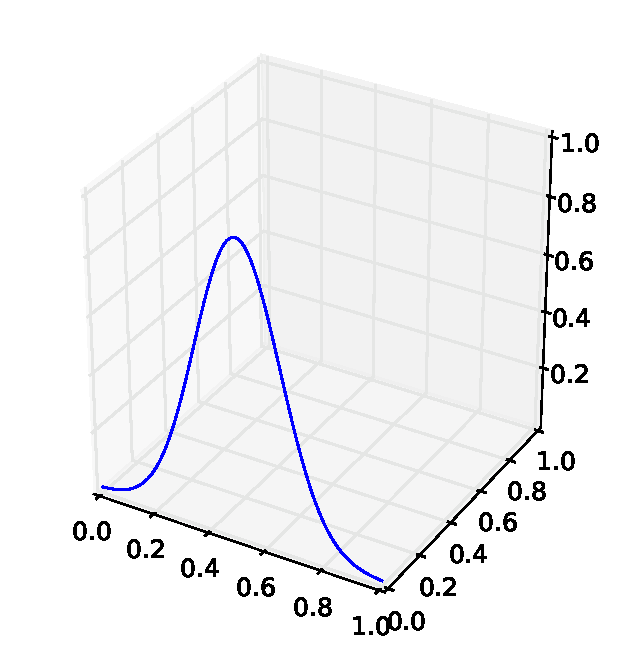
\includegraphics[width=3cm]{figures/python/newfromold-sum2-k1}
\end{column}
\begin{column}{2mm}
$\times $
\end{column}
\begin{column}{3cm}
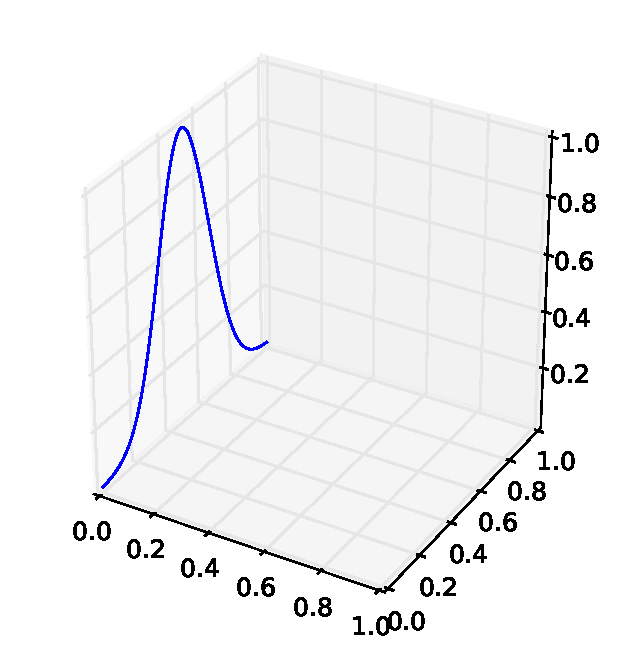
\includegraphics[width=3cm]{figures/python/newfromold-sum2-k2}
\end{column}
\begin{column}{2mm}
$=$
\end{column}
\begin{column}{3cm}
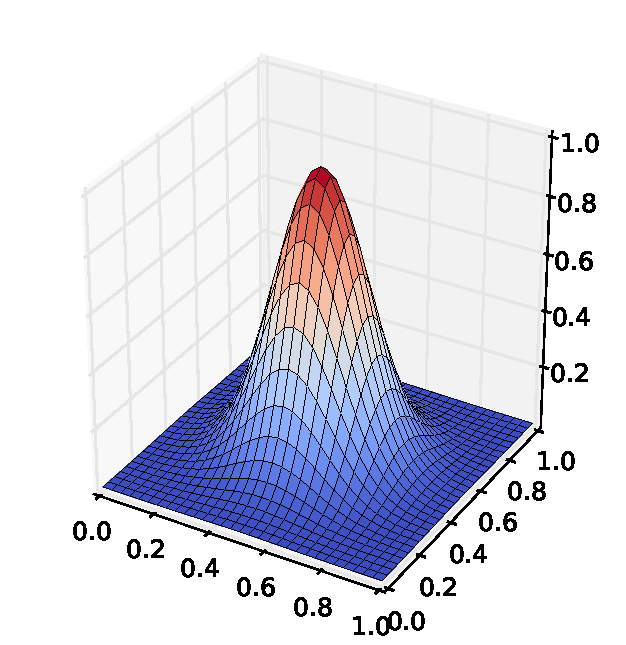
\includegraphics[width=3cm]{figures/python/newfromold-prod2-k12}
\end{column}
\end{columns}
\vspace{5mm}
Calculation shows this is the usual 2D squared exponential kernel.
\end{example}
\end{frame}

% \subsection{Composition with a function}

%%%%%%%%%%%%%%%%%%%%%%%%%%%%%%%%%%%%%%%%%%%%%%%%%%%%%%
\begin{frame}{Composition with a function}
\begin{block}{Property}
Let $k_1$ be a kernel over $D_1 \times D_1$ and $f$ be an arbitrary function $D \rightarrow D_1$, then
\begin{equation*}
k(x,y) = k_1(f(x),f(y))
\end{equation*}
is a kernel over $D \times D $.\\
\small
\textbf{proof}\\
\begin{equation*}
\sum \sum a_i  a_j k(x_i,x_j) = \sum \sum a_i a_j k_1(\underbrace{f(x_i)}_{y_i},\underbrace{f(x_j)}_{y_j}) \geq 0 
\end{equation*}
\end{block}
\vspace{5mm}
\structure{Remarks:}
\begin{itemize}
\item $k$ corresponds to the covariance of $Z(x) = Z_1(f(x))$
\item This can be seen as a (non-linear) rescaling of the input space
\end{itemize}
\end{frame}

%%%%%%%%%%%%%%%%%%%%%%%%%%%%%%%%%%%%%%%%%%%%%%%%%%%%%%
\begin{frame}{}
\begin{example}
We consider $f(x) = \frac1x$ and a Mat\'ern 3/2 kernel $k_1(x,y) = (1 + |x-y|) e^{-|x-y|}$.\\ \vspace{5mm}
\textbf{We obtain:}
\begin{columns}[c]
\begin{column}{5cm}
\begin{center}
Kernel
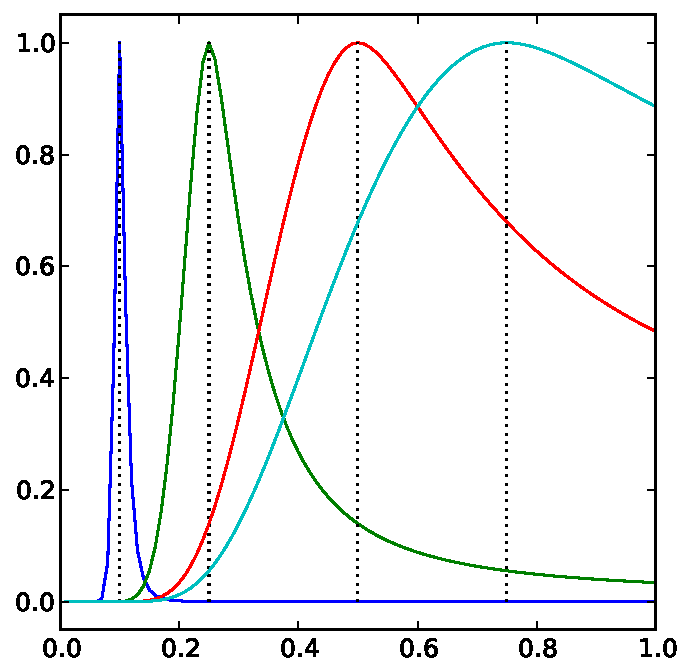
\includegraphics[width=4cm]{figures/python/newfromold-compfunc-k}
\end{center}
\end{column}
\begin{column}{5cm}
\begin{center}
Sample paths
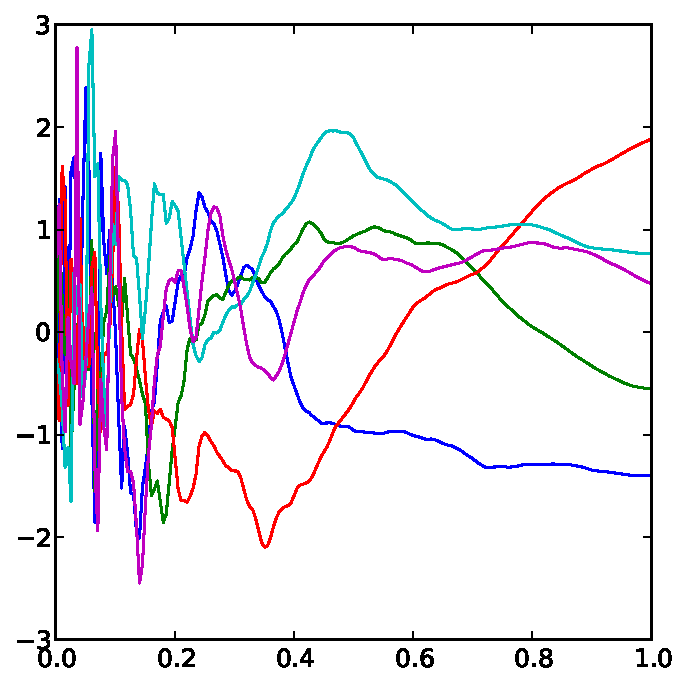
\includegraphics[width=4cm]{figures/python/newfromold-compfunc-traj}
\end{center}
\end{column}
\end{columns}
\end{example}
\end{frame}

%%%%%%%%%%%%%%%%%%%%%%%%%%%%%%%%%%%%%%%%%%%%%%%%%%%%%%
\begin{frame}{}
\structure{All these transformations can be combined!}
\begin{example}
$k(x,y) = f(x)f(y)k_1(x,y)$ is a valid kernel.\\
\vspace{0.5cm}
This can be illustrated with $f(x) = \frac1x$ and $k_1(x,y) = (1 + |x-y|) e^{-|x-y|}$:\\ 
\begin{columns}[c]
\begin{column}{5cm}
\begin{center}
Kernel
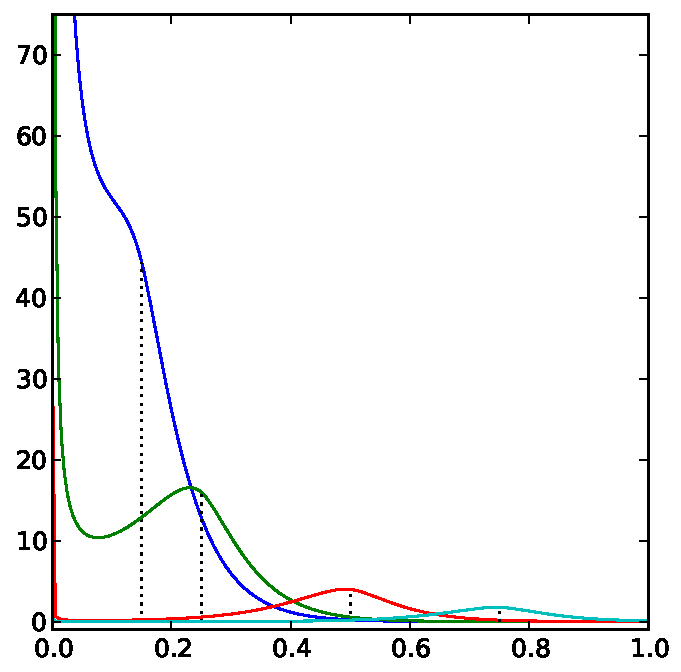
\includegraphics[width=4cm]{figures/python/newfromold-prodfunc-k}
\end{center}
\end{column}
\begin{column}{5cm}
\begin{center}
Sample paths
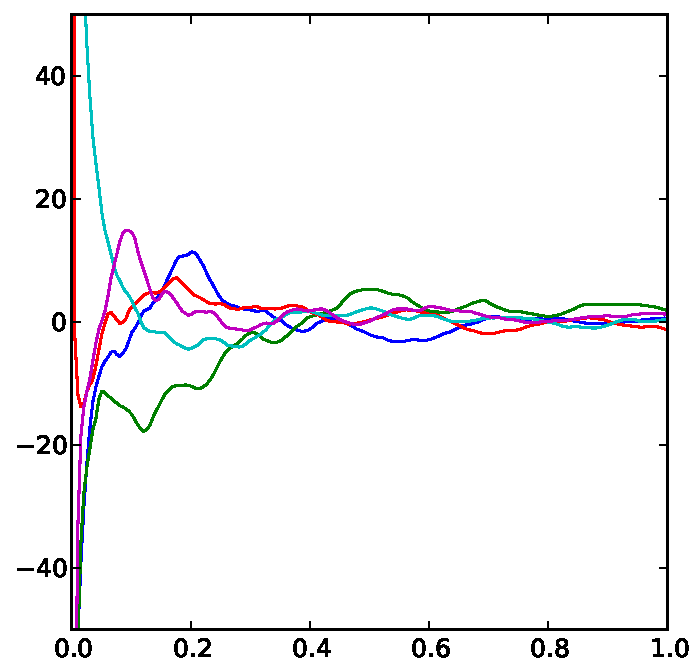
\includegraphics[width=4cm]{figures/python/newfromold-prodfunc-traj}
\end{center}
\end{column}
\end{columns}
\end{example}
\end{frame}


%%%%%%%%%%%%%%%%%%%%%%%%%%%%%%%%%%%%%%%%%%%%%%%%%%%%%%%%%%%%
%%%%%%%%%%%%%%%%%%%%%%%%%%%%%%%%%%%%%%%%%%%%%%%%%%%%%%%%%%%%
\section[Bochner]{Bochner's theorem}
\subsection{}

%%%%%%%%%%%%%%%%%%%%%%%%%%%%%%%%%%%%%%%%%%%%%%%%%%%%%%%%%%%%
% \subsection{Bochner's theorem}

%%%%%%%%%%%%%%%%%%%%%%%%%%%%%%%%%%%%%%%%%%%%%%%%%%%%%%
\begin{frame}{}
\begin{theorem}[Bochner]
A continuous stationary function $k(x,y)=\tilde{k}(x-y)$ is positive definite if and only if $\tilde{k}$ is the Fourier transform of a finite positive measure:
\begin{equation*}
\tilde{k}(t) = \int_\mathds{R} e^{-i \omega t} \mathrm{d} \mu(\omega)
\end{equation*}
\end{theorem}
\vspace{5mm}
This result is very useful to prove the positive definiteness of stationary functions. 
\end{frame}

%%%%%%%%%%%%%%%%%%%%%%%%%%%%%%%%%%%%%%%%%%%%%%%%%%%%%%
\begin{frame}{}
\begin{example}
\begin{columns}[c]
\begin{column}{7cm}
\ \\ \  \\
We consider the following measure:\\
\vspace{2.3cm}
Its Fourier transform gives $\tilde{k}(t) = \displaystyle \frac{\sin(t)}{t}$ :
\end{column}
\begin{column}{5cm}
\begin{center}
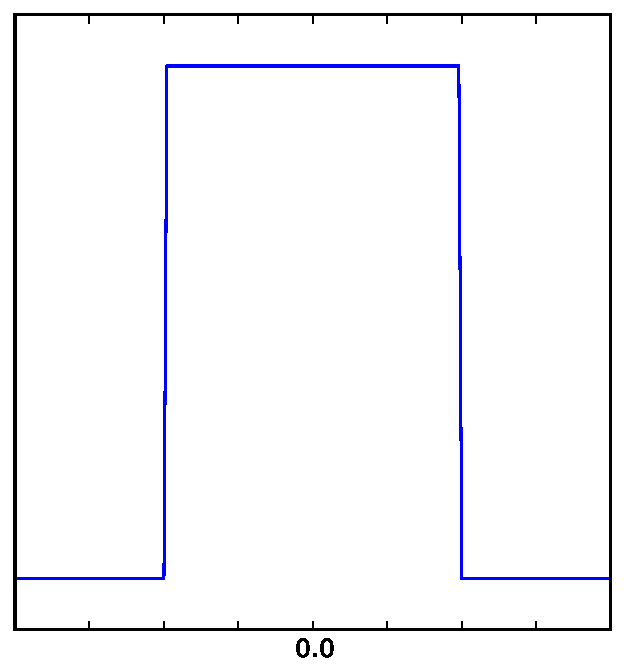
\includegraphics[width=2.5cm]{figures/python/Bochner-musinc}
\end{center}

\begin{center}
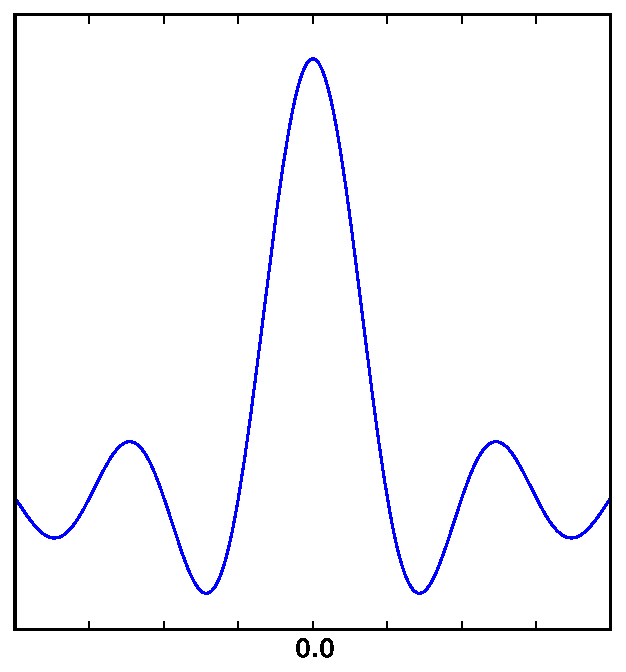
\includegraphics[width=2.5cm]{figures/python/Bochner-ksinc}
\end{center}
\end{column}
\end{columns} 
\vspace{2mm}
As a consequence, $\displaystyle k(x,y) = \frac{\sin(x-y)}{x-y}$
is a valid covariance function.
\end{example}

\end{frame}

%%%%%%%%%%%%%%%%%%%%%%%%%%%%%%%%%%%%%%%%%%%%%%%%%%%%%%
\begin{frame}{}
Bochner theorem can be used to prove the positive definiteness of many usual stationary kernels \vspace{2mm}
\begin{itemize}
  \item The Gaussian is the Fourier transform of itself \\
  \qquad $\Rightarrow$ it is psd.
  \item Matern kernels are the Fourier transforms of $\frac{1}{(1+\omega^2)^p}$ \\
  \qquad $\Rightarrow$ they are psd.
  \item the constant function is the Fourier transform of $\delta_{x,y}$ \\
  \qquad $\Rightarrow$ it is psd.
\end{itemize} \vspace{5mm}
% It can also be generalised to distributions: \vspace{2mm}
% \begin{itemize}
%   \item $\delta_{x,y}$ is the Fourier transform of the constant function \\
%   \qquad $\Rightarrow$ it is psd.
% \end{itemize}
\end{frame}

%%%%%%%%%%%%%%%%%%%%%%%%%%%%%%%%%%%%%%%%%%%%%%%%%%%%%%
\begin{frame}{Spectral approximation with a mixture of Gaussian (A. Wilson, ICML 2013)}
The inverse Fourier transform of a (symmetrised) non centred Gaussian is:
\begin{columns}[c]
\begin{column}{5cm}
\begin{center}
$\mu(\omega)$ \\
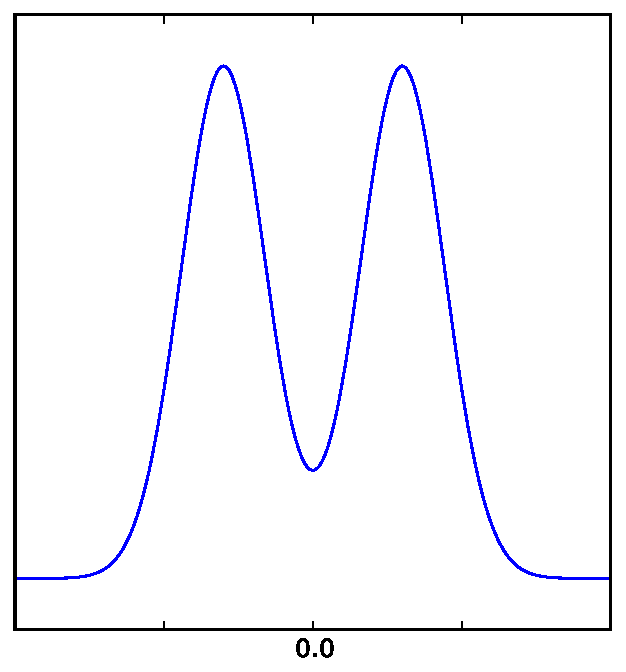
\includegraphics[width=3cm]{figures/python/Bochner-wilsonmu}
\end{center}
\end{column}
\begin{column}{2cm}
\begin{center}
$\stackrel{\longrightarrow}{\mathcal{F}}$
\end{center}
\end{column}
\begin{column}{5cm}
\begin{center}
$\tilde{k}(t)$\\
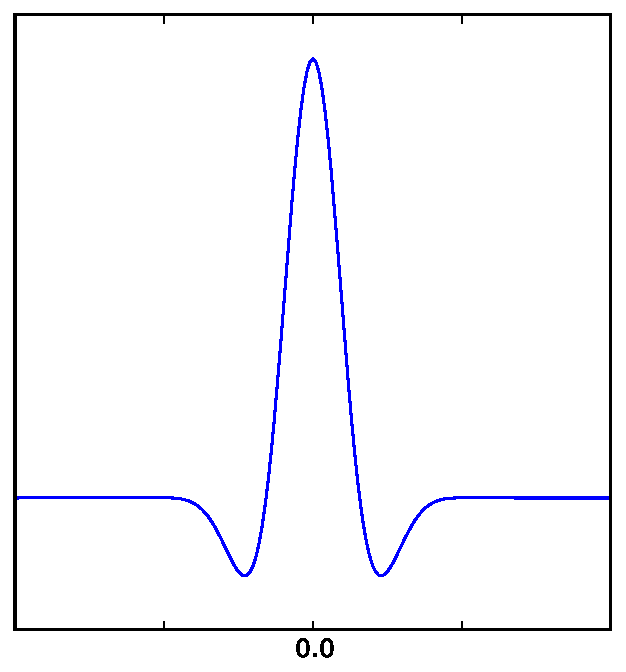
\includegraphics[width=3cm]{figures/python/Bochner-wilsonk}
\end{center}
\end{column}
\end{columns}
\vspace{3mm}
This can be generalised to a measure based on the sum of Gaussians.

\end{frame}

%%%%%%%%%%%%%%%%%%%%%%%%%%%%%%%%%%%%%%%%%%%%%%%%%%%%%%
\begin{frame}{Spectral approximation with a mixture of Gaussian (A. Wilson, ICML 2013)}
We obtain a kernel that is parametrised by the means and the bandwidths of Gaussian bells in the measure space:
\begin{columns}[c]
\begin{column}{5cm}
\begin{center}
$\mu(\omega)$ \\
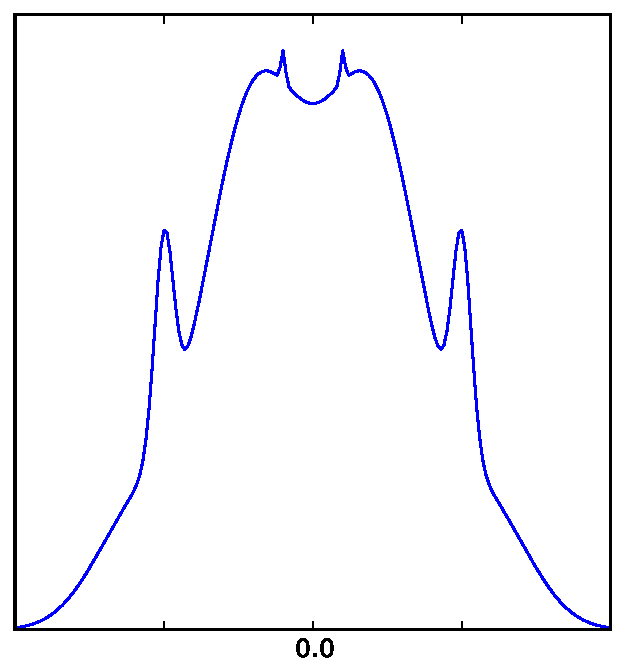
\includegraphics[width=3cm]{figures/python/Bochner-wilsonmus}
\end{center}
\end{column}
\begin{column}{2cm}
\begin{center}
$\stackrel{\longrightarrow}{\mathcal{F}}$
\end{center}
\end{column}
\begin{column}{5cm}
\begin{center}
$\tilde{k}(t)$\\
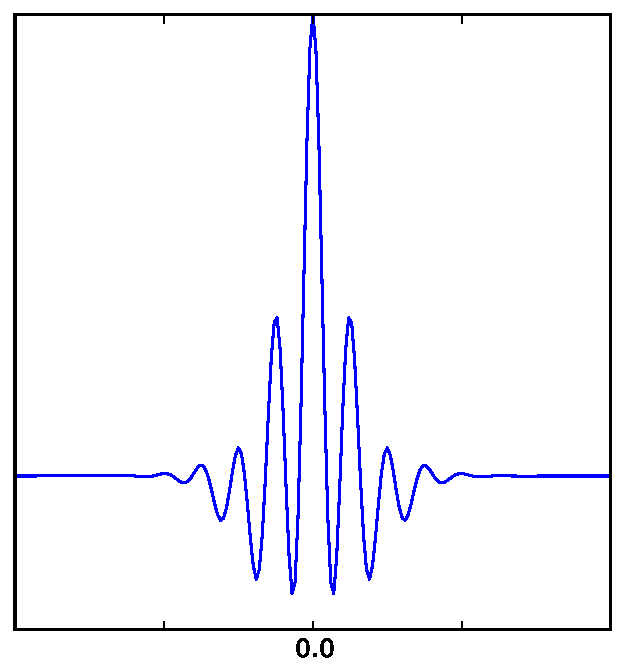
\includegraphics[width=3cm]{figures/python/Bochner-wilsonks}
\end{center}
\end{column}
\end{columns}

\end{frame}

%%%%%%%%%%%%%%%%%%%%%%%%%%%%%%%%%%%%%%%%%%%%%%%%%%%%%%
\begin{frame}{Spectral approximation with a mixture of Gaussian (A. Wilson, ICML 2013)}
The sample paths have the following aspect:\\
\vspace{5mm}
\begin{center}
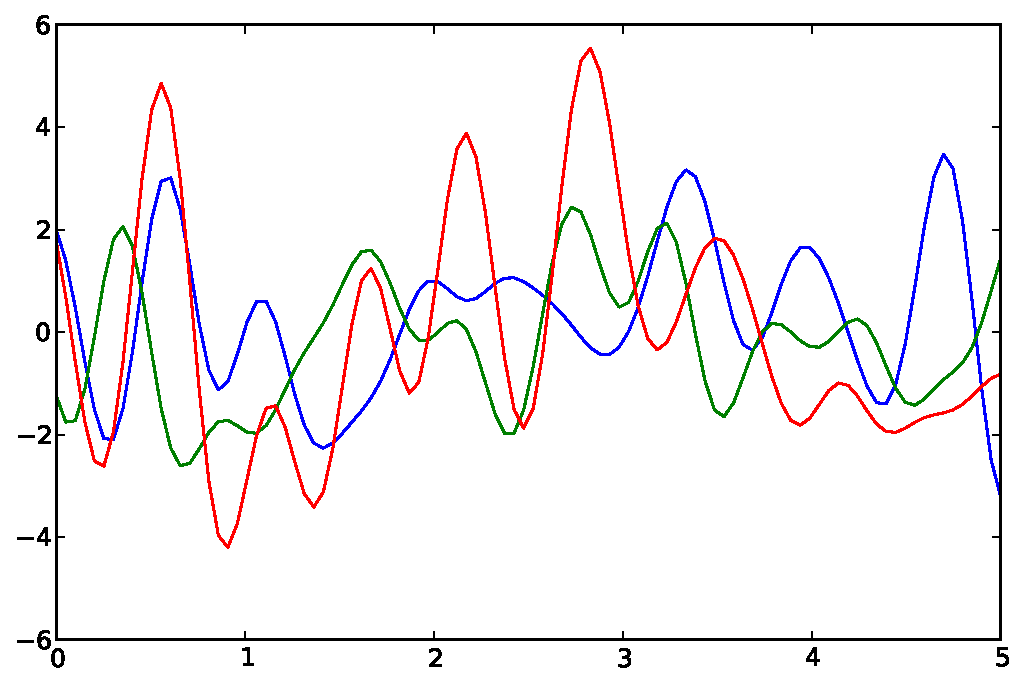
\includegraphics[height=4cm]{figures/python/Bochner-wilsonktraj}
\end{center}
\end{frame}


%%%%%%%%%%%%%%%%%%%%%%%%%%%%%%%%%%%%%%%%%%%%%%%%%%%%%%%%%%%%%%%%%%%%%%%%%%%%%%%%%%%%
%%%%%%%%%%%%%%%%%%%%%%%%%%%%%%%%%%%%%%%%%%%%%%%%%%%%%%%%%%%%%%%%%%%%%%%%%%%%%%%%%%%%
\section[Linear operator]{Effect of a linear operator}
\subsection{}

%%%%%%%%%%%%%%%%%%%%%%%%%%%%%%%%%%%%%%%%%%%%%%%%%%%%%%
\begin{frame}{Effect of a linear operator}
\begin{block}{Property}
Let $L$ be a linear operator that commutes with the covariance, then
$k(x,y) = L_x(L_y(k_1(x,y)))$ is a kernel.
\end{block}
\begin{example}
  We want to approximate a function $[0,1] \rightarrow \mathds{R}$ that is symmetric with respect to $0.5$.
We will consider 2 linear operators:
\begin{equation*}
 L_1 : f(x) \rightarrow 
\left\{ 
\begin{aligned}
 f(x) \text{\qquad}  & x < 0.5 \\
 f(1-x) \text{\qquad}   & x \geq 0.5 
\end{aligned}
\right.
\end{equation*}
$$ L_2 : f(x) \rightarrow \frac{f(x) + f(1-x)}{2}.$$
\textbf{Exercice:} Compute the kernel associated to the second operator.
\end{example}
\end{frame}

%%%%%%%%%%%%%%%%%%%%%%%%%%%%%%%%%%%%%%%%%%%%%%%%%%%%%%
\begin{frame}{Effect of a linear operator: example [Ginsbourger 2013]}
Examples of associated sample paths are 

\begin{columns}[c]
\begin{column}{5cm}
\begin{center}
 $k_1 = L_1(L_1(k))$
\end{center}
 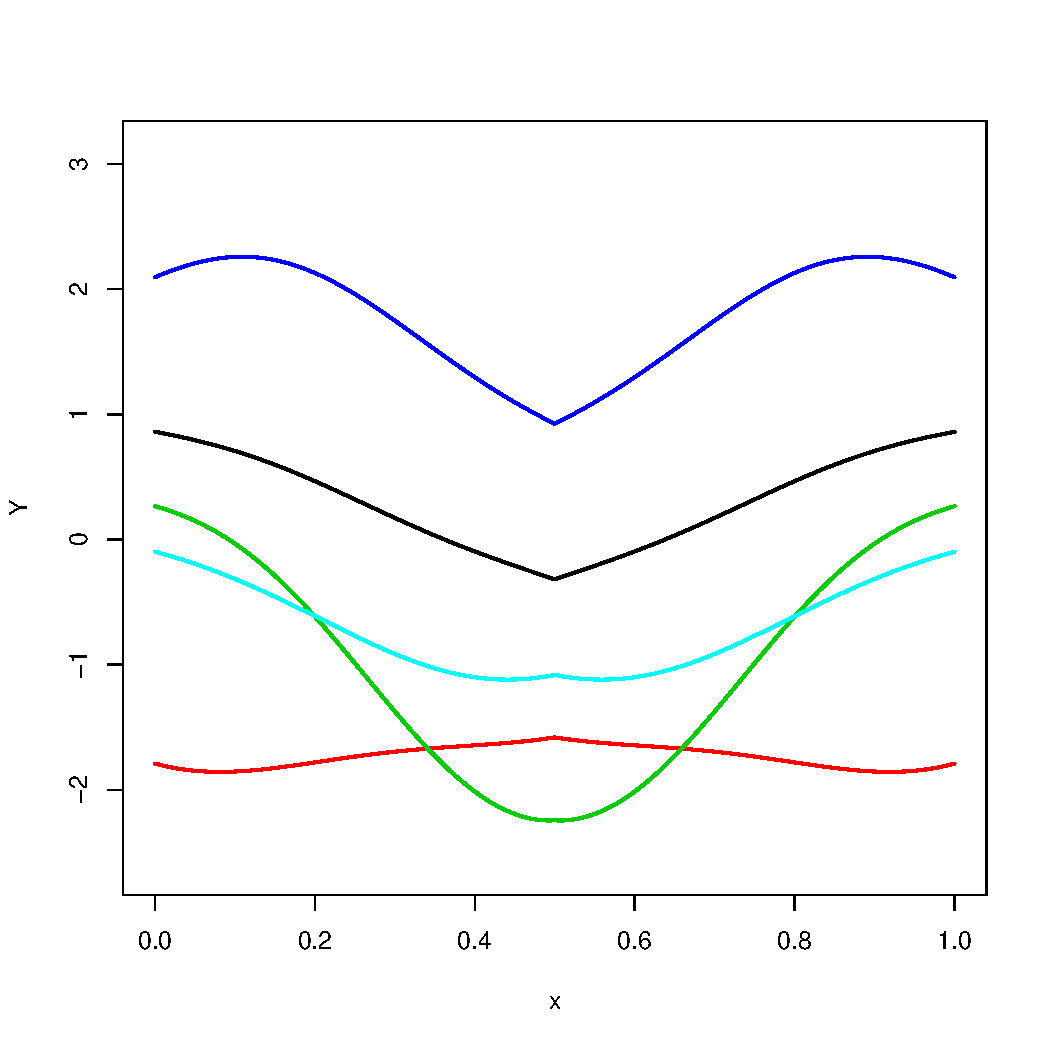
\includegraphics[height=5cm]{figures/R/p2-sym1}
\end{column}
\begin{column}{5cm}
\begin{center}
 $k_2= L_2(L_2(k))$
\end{center}
 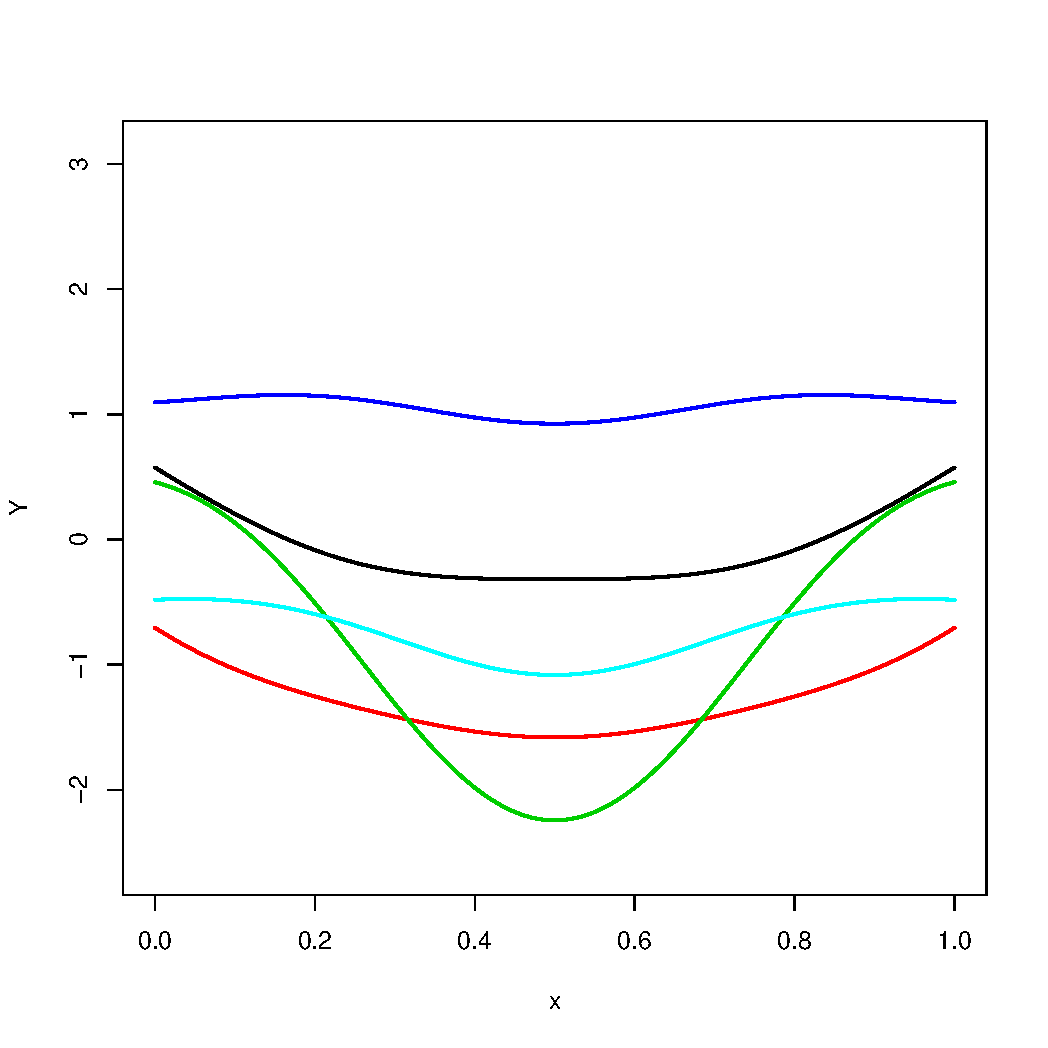
\includegraphics[height=5cm]{figures/R/p2-sym2}
\end{column}
\end{columns}
The differentiability is not always respected!
\end{frame}

%%%%%%%%%%%%%%%%%%%%%%%%%%%%%%%%%%%%%%%%%%%%%%%%%%%%%%
\begin{frame}{Effect of a linear operator}
These linear operator are projections onto a space of symmetric functions:
\begin{center}
\vspace{0.5cm}
 \includegraphics[height=2cm]{figures/latexdraw/proj-sym}
\vspace{0.5cm}
\end{center}
Is there an optimal projection?\\
\vspace{0.5cm}
\alert{$\Rightarrow$ This can be difficult... but it raises interesting questions!}
\end{frame}

%%%%%%%%%%%%%%%%%%%%%%%%%%%%%%%%%%%%%%%%%%%%%%%%%%%%%%
\begin{frame}{Effect of a linear operator}
Can we construct a GP such that the integrals of the paths are null?\\ \vspace{3mm}
We can think of the following application:
$$ L : f(x) \rightarrow f(x) - \int f(s) \dx s.$$
More generally, for all $g: [0,1] \rightarrow \mathds{R}$, the application
$$ L_g : f(x) \rightarrow f(x) - \frac{g(x)}{\int g(s) \dx s}\int f(s) \dx s$$
will center $f$. It turns out that the optimal $g$ is $g(x) =\int k(x,s) \dx s$
% $$ g(x) = \frac{\int k(x,s) \dx s}{\iint k(s,t) \dx s \dx s} $$
\begin{exampleblock}{Exercice}
\begin{enumerate}
	\item Compute the associated kernel.
	\item What is the distribution of $Z|\int Z = 0$ ?
\end{enumerate}
\end{exampleblock}
\end{frame}

%%%%%%%%%%%%%%%%%%%%%%%%%%%%%%%%%%%%%%%%%%%%%%%%%%%%%%%%%%%%%%%%%%%%%%%%
\section[Exotic obs.]{Adding ``exotic'' observations}
\subsection{}

%%%%%%%%%%%%%%%%%%%%%%%%%%%%%%%%%%%%%%%%%%%%%%%%%%%%%%
\begin{frame}{}
Up to now, we have only considered regular observation of the kind $f(X)$. \\ \vspace{5mm}
According to what we have just seen, the conditioning can also include observation of the integral. This can be generalised to other linear operators such as the derivative:
$$ Z \ \left| \ Z(X) = F, \int Z = a, \frac{\dx Z}{\dx x}(X')= F' \right. $$
\end{frame}

%%%%%%%%%%%%%%%%%%%%%%%%%%%%%%%%%%%%%%%%%%%%%%%%%%%%%%
\begin{frame}{}
\begin{example}
	If we take into account that the function is centred, we obtain:
	\begin{center}
	\includegraphics[height=6cm]{figures/R/exotic_int}
	\end{center}
\end{example}
\end{frame}

%%%%%%%%%%%%%%%%%%%%%%%%%%%%%%%%%%%%%%%%%%%%%%%%%%%%%%
\begin{frame}{}
\begin{example}
	Whereas if we ignore it:
	\begin{center}
	\includegraphics[height=6cm]{figures/R/exotic_pasint}
	\end{center}
\end{example}
\end{frame}

%%%%%%%%%%%%%%%%%%%%%%%%%%%%%%%%%%%%%%%%%%%%%%%%%%%%%%
\begin{frame}{}
Similarly, we can include in the model some derivatives observations:
	\begin{center}
	\includegraphics[height=6cm]{figures/R/exotic_der}
	\end{center}
\end{frame}

%%%%%%%%%%%%%%%%%%%%%%%%%%%%%%%%%%%%%%%%%%%%%%%%%%%%%%
\begin{frame}{}
We can see interesting behaviour if we look at a model with only derivatives.
	\begin{center}
	\includegraphics[height=6cm]{figures/R/exotic_deronly}
	\end{center}
\end{frame}

%%%%%%%%%%%%%%%%%%%%%%%%%%%%%%%%%%%%%%%%%%%%%%%%%%%%%%
\begin{frame}{}
As always, we can simulate conditional paths:
	\begin{center}
	\includegraphics[height=6cm]{figures/R/exotic_simul}
	\end{center}
\end{frame}

%%%%%%%%%%%%%%%%%%%%%%%%%%%%%%%%%%%%%%%%%%%%%%%%%%%%%%%%%%%%%%%%%%%%%%%%
\section[Concl.]{Conclusion}
\subsection{}

%%%%%%%%%%%%%%%%%%%%%%%%%%%%%%%%%%%%%%%%%%%%%%%%%%%%%%
\begin{frame}{}
\structure{Small Recap} We have seen that \vspace{2mm}
\begin{block}{}
\begin{itemize}
 \item It is possible to build as many kernels as you want
 \begin{itemize}
 	\item Given some data, there is not one GP model but an infinity...
 \end{itemize}
 \item Kernels encode the prior belief on the function to approximate.
 \begin{itemize}
 	\item They can (and should) be tailored to the problem at hand.
 \end{itemize}
 \item It is possible to include more than regular function observations.
 \item If you want the decisions based on your model to be reliable, model validation is of the utmost importance.
\end{itemize}
\end{block}
\end{frame}

%%%%%%%%%%%%%%%%%%%%%%%%%%%%%%%%%%%%%%%%%%%%%%%%%%%%%%
\begin{frame}{}
3 tools for designing new kernels: \vspace{2mm}
\begin{block}{Making new from old}
Various operations can be applied to kernels while keeping the psd :
\begin{columns}[c]
\begin{column}{3.5cm}
\begin{itemize}
 \item sum
 \item product
\end{itemize}
\end{column}
\begin{column}{7cm}
\begin{itemize}
 \item composition with a function
 \item[]
\end{itemize}
\end{column}
\end{columns}
\end{block}
\vspace{2mm}
\begin{block}{Bochner Theorem}
is very useful to prove a stationary kernel is psd.
\end{block}
\vspace{2mm}
\begin{block}{Linear operators}
If we have a linear application that transforms any function into a function satisfying the desired property, it is possible to build a GP fulfilling the requirements.
\end{block}
\end{frame}

%%%%%%%%%%%%%%%%%%%%%%%%%%%%%%%%%%%%%%%%%%%%%%%%%%%%%%%%%%%%%%%%%%%%%%%%%%%%%%%
%%%%%%%%%%%%%%%%%%%%%%%%%%%%%%%%%%%%%%%%%%%%%%%%%%%%%%%%%%%%%%%%%%%%%%%%%%%%%%%
%%%%%%%%%%%%%%%%%%%%%%%%%%%%%%%%%%%%%%%%%%%%%%%%%%%%%%%%%%%%%%%%%%%%%%%%%%%%%%%
%%%%%%%%%%%%%%%%%%%%%%%%%%%%%%%%%%%%%%%%%%%%%%%%%%%%%%%%%%%%%%%%%%%%%%%%%%%%%%%
\end{document}



%%%%%%%%%%%%%%%%%%%%%%%%%%%%%%%%%%%%%%%%%%%%%%%%%%%%%%
%%%%%%%%%%%%%%%%%%%%%%%%%%%%%%%%%%%%%%%%%%%%%%%%%%%%%%
%%%%%%%%%%%%%%%%%%%%%%%%%%%%%%%%%%%%%%%%%%%%%%%%%%%%%%

\structure{}

\begin{center}
  \begin{tabular}{|c|cc|}

  \end{tabular}
\end{center}

###
%%%%%%%%%%%%%%%%%%%%%%%%%%%%%%%%%%%%%%%%%%%%%%%%%%%%%%
\begin{frame}{}

\end{frame}

###
\begin{block}{}

\end{block}

###
\begin{center}
\includegraphics[height=5cm]{figures/}
\end{center}

###
\begin{columns}[c]
\column{5cm}

\column{5cm}

\end{columns}
